\chapter{迁移学习和持续学习的可学习性}
\label{chap:transfer-learning-theory}

设一个邮件过滤器用三月的邮件训练，在三月邮件上的错误率很低。四月到来以后，这份结果还不能回答三个问题。第一，四月的邮件构成改变了，它能否继续识别诈骗邮件？第二，邮件来源不变，但用户改为更在意误拦正常邮件，已有模型能否支持新的拦截决策？第三，邮件按月到来，旧月份的数据随后无法重新读取，模型能否在适应新邮件的同时，继续正确处理再次出现的旧类型邮件？三个问题都要求把有限经验用于总体，但算法能读取的信息和最终接受的评价各不相同。

第~\ref{chap:machine-learning-paradigms}章已经从做法上介绍过这两类范式：迁移学习把来源问题上学到的知识用于目标问题，持续学习让模型随经验陆续到来而更新，同时保住仍然需要的旧能力。那里回答“怎样做”，本章回答“在什么条件下能够证明做得到”。前几章的可学习性结论建立在同一组前提上，回顾第~\ref{sec:risk-comparison}节的风险比较就能看清它们。设候选$h$的总体风险为$R(h)$、经验风险为$\widehat R(h)$。若在一次抽样的成功事件上，全部候选都满足$|R(h)-\widehat R(h)|\leq a$，而算法输出$\widehat h$的经验风险至多比类内最小值高$\rho$，则对每个比较候选$h$，
\begin{equation}
 R(\widehat h)\leq\widehat R(\widehat h)+a
 \leq\widehat R(h)+\rho+a
 \leq R(h)+\rho+2a.
 \label{eq:transfer-iid-comparison}
\end{equation}
这正是定理~\ref{thm:approximate-erm-risk}的三步比较。它悄悄用了三条联系：训练时计分的损失就是评价时的损失；计算经验平均的样本来自评价所用的总体；选择模型时，算法能算出每个候选的经验损失。四月邮件构成改变时，第二条断开，因为$\widehat R$估计的只是三月的风险。误拦代价改变时，第一条断开，旧任务的经验量估计的是另一种风险。旧邮件不能重读时，第三条可能断开，算法无法再检查候选在旧数据上的表现。本章的正面结论都在做同一件事：用明确的额外条件重新接上断开的联系，再使用有限样本的偏差控制。反例则说明，哪些缺口无论增加多少同类样本都补不上。

本章先在第~\ref{sec:transfer-learning-setting}节统一三种变化的描述、可用信息和评价基准，然后在第~\ref{sec:domain-adaptation}、\ref{sec:task-transfer-learnability}、\ref{sec:continual-learnability}节分别固定分布变化、任务变化和历史访问限制三种协议。每一部分都按同一顺序推进：先判断可见信息在原则上是否足以确定所需决策，再构造可以估计的学习目标，最后核算样本、求解误差和存储。全章沿用一个两种邮件的小例子，所有数值都可以手算复核。以下有限样本结论中，样本数与有限候选数均为正整数，失败概率$\delta\in(0,1)$，优化误差非负；涉及的损失、上确界和输出均假定满足可测性要求（第~\ref{sec:measurability-convention}节），需要条件分布时假定相应的条件概率核存在。

\section{学习环境、可用信息与评价目标}
\label{sec:transfer-learning-setting}

回到四月的邮件。同样是“情况变了”，变化可能发生在三个地方：邮件的来源变了，评价预测的方式变了，或者过去的数据不能再读了。在讨论任何保证以前，需要先说清三件事：哪个条件改变了，算法实际能读取什么，最后用什么风险来评价。本节建立这三件事的共同说法；具体的量词、抽样条件和算法约定，在后面三节各自的协议中落实。

\subsection{分布变化、任务变化与历史访问限制}
\label{sec:transfer-change-types}

先固定输入空间$X$、标签空间$Y$和取值于$[0,1]$的损失。沿用第~\ref{chap:machine-learning-paradigms}章的说法，提供已有带标签数据的环境称为\term{源域}（source domain），希望模型最终生效的环境称为\term{目标域}（target domain）。在理论分析中，一个域由输入与标签的联合分布刻画，源域和目标域分别记为$\mathcal P_S,\mathcal P_T$。三月是源域，四月是目标域；邮件仍分为“正常”与“诈骗”，两类错误的计分方式也不变。改变的只有联合分布：某类邮件出现得更频繁，诈骗邮件占比上升，或者同一类邮件是否属于诈骗的规律改变。这是\emph{分布变化}。

另一种变化保持完整观测的生成分布$\mathcal P$不变，只改变计分方式。原来漏判一封诈骗邮件与误拦一封正常邮件代价相同，现在用户更在意误拦：误拦记0.8，漏判记0.2。邮件、标签及其联合分布都没有变，最优决策却可能改变。我们用同一个$\mathcal P$与两个损失$\ell_S,\ell_T$表达这一情形，称为\emph{任务变化}。两种变化互不蕴含：四月来源改变时，可以仍用原来的损失；来源不变时，也可以换一种损失。

第三个条件是历史数据能否再次读取。邮件按月到来，系统每月更新一次，旧月份的数据随后被删除或不再允许访问。持续到达的数据本身可以同时伴随分布变化或任务变化；第~\ref{sec:continual-learnability}节先固定任务，单独研究访问限制。若标签的定义也改变了，例如从识别诈骗改为识别邮件主题，就要先固定底层的邮件来源，再分别说明每个任务的标签怎样从同一封邮件产生；两个任务共用记号$y$，并不说明它们的联合分布相同。表~\ref{tab:transfer-three-changes}汇总三种变化各自固定了什么、改变了什么。

\begin{table}[htbp]
 \centering
 \caption{三种变化的对照。每一行固定其余条件，只改变一项；实际问题可以同时出现多项变化。}
 \label{tab:transfer-three-changes}
 \begin{tabularx}{\linewidth}{@{}l>{\raggedright\arraybackslash}X>{\raggedright\arraybackslash}X>{\raggedright\arraybackslash}X@{}}
  \toprule
  变化 & 保持不变 & 发生改变 & 邮件例子 \\
  \midrule
  分布变化 & 输入、标签的含义与损失 & 联合分布$\mathcal P_S\to\mathcal P_T$ & 四月促销邮件变多 \\
  任务变化 & 完整观测的分布$\mathcal P$ & 损失$\ell_S\to\ell_T$ & 误拦代价从0.5升为0.8 \\
  历史访问限制 & 任务；各阶段分布可变可不变 & 旧数据不能重读 & 三月邮件在四月被删除 \\
  \bottomrule
 \end{tabularx}
\end{table}

\subsection{目标反馈与可保留的信息}
\label{sec:transfer-feedback-information}

模型能否适应四月，很大程度上取决于算法能看到四月的哪些信息。目标反馈可以分成三档：带标签的目标样本、无标签的目标输入、训练时完全没有目标数据。若训练时可以使用目标数据，哪怕没有标签，这类问题称为\term{领域自适应}（domain adaptation）；只给目标输入、不给目标标签的情形称为\term{无监督领域自适应}（unsupervised domain adaptation）。四月邮件已经到达、还没人逐封标注，就是后者。若训练和模型选择时都拿不到任何目标数据，只能要求模型直接用于事先允许的新环境，这类问题称为\term{领域泛化}（domain generalization）。部署后模型当然要读取每封待预测的邮件，但读取一个输入作出预测，与用一批目标数据更新或选择模型，是两种不同的信息访问；只有后者属于领域自适应。后面每条风险保证都必须与它所假定的反馈协议一致。

无标签目标输入能提供什么，可以用一个具体情形看清。系统收到四月邮件的词频统计，却不知道这些邮件是否诈骗。它能比较“优惠”一词在三月和四月出现得多频繁，却不能仅凭频率变化判断这个词与诈骗的关系是否也变了。允许查询少量四月标签时，原本无法区分的规律可能被区分；连四月输入也拿不到时，只能依靠训练前规定的新环境范围。同样是“适应四月”，反馈不同，能证明的结论也不同。

第二组区分发生在旧阶段留下的东西上。原始数据可以重访时，后续算法可以按需要重新计算任何量；不能重访时，算法只拥有保留下来的知识或状态。这些载体保留的信息差别很大：一个只输出类别的分类器只说明“这封邮件更可能是哪一类”；一个概率模型还说明“有多大把握”；一个特征映射保留了某些输入之间的区别，丢掉了另一些；对每个候选累计的错误数，则只够回答某一类事先确定的比较问题。第~\ref{sec:task-transfer-learnability}节会看到，只保存类别会丢掉新代价所需的概率信息；第~\ref{sec:continual-learnability}节会看到，累计错误数足以支持固定候选的历史选择，却不能评价以后新增的候选。因此，源样本数、目标反馈数和存储预算要分别计数。已经有一个模型，并不意味着训练它的旧数据仍然可用。

\subsection{风险基准与迁移收益}
\label{sec:transfer-risk-benchmarks}

说清信息以后，还要固定评价对象。迁移问题评价目标分布上的风险$R_T$；持续学习可以评价各历史阶段风险的平均，也可以要求每个历史阶段都接近各自的最优值。每种评价都要说明允许怎样的预测器，以及与哪个候选空间中的最优者比较。比较基准的差别可以很大。设三月的邮件全是输入$a$且标签为0，四月的邮件也全是$a$但标签为1。若只允许一个确定性分类器同时承担两个月的预测，它在$a$上只能给出一个类别，两个月的平均风险至少为$1/2$；若允许每个月各用自己的分类器，平均最优风险为0。前者是“同一模型”的基准，后者是“各月分别选模型”的基准，推导中途不能把一个换成另一个。

另一组需要分开的判断是“能学会”与“迁移有收益”。若四月可以不断取得独立的标签，而目标候选空间本来就PAC可学习，那么忽略三月的知识、直接用四月标签重新学习，就已经能学会。迁移理论需要进一步说明：在目标标签缺少或预算有限时，旧知识提供了什么额外约束；若声称它节省了新标签或计算，还应在相同目标风险和可比预算下，与直接学习比较。

持续学习还关心另一种“收益”：更新以后，旧能力保住了多少。吸收新数据、改善当前预测的要求称为\term{可塑性}（plasticity），保持仍然有用的历史能力的要求称为稳定性（stability）。这里的稳定性比较的是\emph{同一学习过程在不同时间}输出的模型，在\emph{同一个历史分布}上的风险变化，第~\ref{sec:continual-learnability}节用遗忘量$F_{i,t}$度量它。第~\ref{sec:algorithmic-stability}节的算法稳定性比较的则是\emph{同一时刻}在两份只相差一个样本的训练集上得到的输出，回答输出是否过度依赖个别样本。前者可以在算法稳定性很好的情况下失败，例如每月都用一个对单个样本不敏感的算法、却只拟合当月数据；后者也可以在毫无遗忘的情况下很差，例如算法强烈依赖个别样本，但旧阶段的风险恰好没有上升。两种性质都有用，回答的却是不同问题，下文不混用。
\section{分布变化下的迁移学习}
\label{sec:domain-adaptation}

现在固定任务和损失，只让邮件来源从三月变成四月。三月上的低错误率可能说明分类规律已经学对，也可能只说明模型擅长处理三月常见的邮件；四月提高了另一类邮件的比例后，两种情形的后果不同。本节先问源观测与目标决策之间缺少什么联系（第~\ref{sec:transfer-identifiability}节），再按目标数据是否可用组织正面结论。有无标签目标输入时，第~\ref{sec:adaptation-risk}节给出三条路线：协变量偏移下按输入重加权，标签偏移下按类别重加权，以及用两个分类器的预测分歧给出目标风险上界；它们使用不同的跨域联系，条件和统计代价分别核对。完全没有目标数据时，第~\ref{sec:domain-generalization}节另行规定评价新环境的方式。

\subsection{分布偏移与目标可识别性}
\label{sec:transfer-identifiability}

本小节固定任务和损失，说明变化发生在联合分布的哪一部分、算法看到什么，以及这些信息是否足以选出目标上的好决策。偏移的名称只描述两个分布之间的关系，本身不给出学习保证。

\subsubsection{联合分布的变化与偏移类型}
\label{sec:distribution-shift}

若源域与目标域的联合分布可以任意不同，源数据就无法告诉我们目标域的任何事情；迁移要成立，两个分布必须有某一部分保持不变。为了说清“哪一部分不变”，把联合分布拆成两个因子。它可以写成输入分布与条件标签分布之积，也可以写成类别比例与类内输入分布之积：
\begin{equation}
 \mathcal P(x,y)=\mathcal P^X(x)\,\mathcal P(y\mid x)
               =\mathcal P^Y(y)\,\mathcal P(x\mid y).
 \label{eq:transfer-two-factorizations}
\end{equation}
一般情形中，乘积表示边缘分布与条件概率核的组合，离散情形直接按概率相乘。第一种分解中，$\mathcal P^X$描述各种邮件出现得多频繁，$\mathcal P(y\mid x)$描述看到某种邮件后它是诈骗的概率；二分类时记$\eta(x)=\mathbb P(y=1\mid x)$。第二种分解中，$\mathcal P^Y$描述诈骗邮件占多大比例，$\mathcal P(x\mid y)$描述诈骗邮件和正常邮件各自长什么样。

用一个可以手算的例子看两种分解。邮件只有两种：$a$表示普通通知，$b$表示含链接的促销邮件，$y=1$表示诈骗。两个月都满足$\eta(a)=0.1$、$\eta(b)=0.9$；三月中$a,b$的比例为$0.9,0.1$，四月则为$0.1,0.9$。以下数值均为教学构造。图~\ref{fig:lt9-joint-factorizations}把每个月的联合分布同时写成两种分解。按第一种分解读，两个月只有输入比例不同，条件标签概率完全相同。按第二种分解读，三月的诈骗比例为$0.9\times0.1+0.1\times0.9=0.18$，四月为$0.82$；诈骗邮件中$a$所占的比例在三月是$0.09/0.18=1/2$，四月是$0.01/0.82=1/82$。同一对分布，在第二种分解下两个因子都变了。

\begin{figure*}[htbp]
 \centering
 % 第9章：同一联合分布的两种分解（教学构造，数值可逐格复算）。
% 两种邮件 a（普通通知）、b（含链接促销），y=1 表示诈骗。
% 三月（源域）：P^X(a)=0.9, P^X(b)=0.1；四月（目标域）：P^X(a)=0.1, P^X(b)=0.9。
% 两个月都有 eta(a)=P(y=1|a)=0.1, eta(b)=0.9。
% 联合概率 P(x,y)=P^X(x)eta：三月 (a,0)=.81 (a,1)=.09 (b,0)=.01 (b,1)=.09；
% 四月 (a,0)=.09 (a,1)=.01 (b,0)=.09 (b,1)=.81。
% 类别比例：三月 P^Y(1)=.18，四月 .82；类内分布 P(x|y)=P(x,y)/P^Y(y)：
% 三月 P(a|0)=.81/.82=81/82, P(b|0)=1/82, P(a|1)=P(b|1)=1/2；
% 四月 P(a|0)=1/2, P(a|1)=1/82, P(b|1)=81/82。
\begingroup
\definecolor{FigureGreen}{HTML}{829C8B}
\definecolor{FigureGreenFill}{HTML}{E8EEE9}
\newcommand{\ltNineCell}[5]{%
  \node[draw=FigureGrid,fill=#5,minimum width=#3 mm,minimum height=6.4mm,
    inner sep=0pt,anchor=north west,font=\figurefont\footnotesize]
    at (#1,#2) {#4};}
\begin{tikzpicture}[figure picture,x=1mm,y=1mm]
\foreach \row/\top/\name/\pa/\pb/\jaz/\jao/\jbz/\jbo/\pyz/\pyo/\az/\bz/\ao/\bo in {%
  0/60/三月（源域）/0.9/0.1/0.81/0.09/0.01/0.09/0.82/0.18/{81/82}/{1/82}/{1/2}/{1/2},%
  1/27/四月（目标域）/0.1/0.9/0.09/0.01/0.09/0.81/0.18/0.82/{1/2}/{1/2}/{1/82}/{81/82}}{%
  \node[figure heading,anchor=west] at (0,\top+4.5) {\name};
  % 左块：输入比例与条件标签概率
  \ltNineCell{0}{\top}{12}{$x$}{white}
  \ltNineCell{12}{\top}{15}{$\mathcal P^X(x)$}{white}
  \ltNineCell{27}{\top}{15}{$\eta(x)$}{white}
  \ltNineCell{0}{\top-6.4}{12}{$a$}{white}
  \ltNineCell{12}{\top-6.4}{15}{\pa}{FigureRedFill}
  \ltNineCell{27}{\top-6.4}{15}{0.1}{FigureGreenFill}
  \ltNineCell{0}{\top-12.8}{12}{$b$}{white}
  \ltNineCell{12}{\top-12.8}{15}{\pb}{FigureRedFill}
  \ltNineCell{27}{\top-12.8}{15}{0.9}{FigureGreenFill}
  % 中块：联合分布
  \ltNineCell{62}{\top}{12}{}{white}
  \ltNineCell{74}{\top}{14}{$y=0$}{white}
  \ltNineCell{88}{\top}{14}{$y=1$}{white}
  \ltNineCell{62}{\top-6.4}{12}{$a$}{white}
  \ltNineCell{74}{\top-6.4}{14}{\jaz}{FigureBlueFill}
  \ltNineCell{88}{\top-6.4}{14}{\jao}{FigureBlueFill}
  \ltNineCell{62}{\top-12.8}{12}{$b$}{white}
  \ltNineCell{74}{\top-12.8}{14}{\jbz}{FigureBlueFill}
  \ltNineCell{88}{\top-12.8}{14}{\jbo}{FigureBlueFill}
  % 右块：类别比例与类内输入分布
  \ltNineCell{122}{\top}{11}{$y$}{white}
  \ltNineCell{133}{\top}{14}{$\mathcal P^Y(y)$}{white}
  \ltNineCell{147}{\top}{17}{$\mathcal P(a\mid y)$}{white}
  \ltNineCell{122}{\top-6.4}{11}{0}{white}
  \ltNineCell{133}{\top-6.4}{14}{\pyz}{FigureRedFill}
  \ltNineCell{147}{\top-6.4}{17}{\az}{FigureRedFill}
  \ltNineCell{122}{\top-12.8}{11}{1}{white}
  \ltNineCell{133}{\top-12.8}{14}{\pyo}{FigureRedFill}
  \ltNineCell{147}{\top-12.8}{17}{\ao}{FigureRedFill}
  % 箭头：联合分布分别分解
  \draw[figure flow] (61,\top-9.6) -- (43,\top-9.6);
  \draw[figure flow] (103,\top-9.6) -- (121,\top-9.6);
}
\node[figure note] at (21,73.5) {输入比例 $\times$ 条件标签};
\node[figure note] at (82,73.5) {联合分布 $\mathcal P(x,y)$};
\node[figure note] at (143,73.5) {类别比例 $\times$ 类内分布};
% 图例
\node[draw=FigureGrid,fill=FigureGreenFill,minimum width=4mm,minimum height=3mm,inner sep=0pt] at (30,-2) {};
\node[figure note,anchor=west] at (33,-2) {两个月相同};
\node[draw=FigureGrid,fill=FigureRedFill,minimum width=4mm,minimum height=3mm,inner sep=0pt] at (70,-2) {};
\node[figure note,anchor=west] at (73,-2) {两个月不同};
\node[figure note,anchor=west] at (100,-2) {$\mathcal P(b\mid y)=1-\mathcal P(a\mid y)$};
\end{tikzpicture}
\endgroup

 \caption{同一联合分布的两种分解。每行中间是该月的联合概率表，左侧按“输入比例$\times$条件标签概率”分解，右侧按“类别比例$\times$类内分布”分解；绿色格在两个月相同，红色格不同。两个月的$\eta(x)$相同，所以这是协变量偏移；但类内分布$\mathcal P(a\mid y)$也改变了，所以它不是标签偏移。数值为教学构造，可由$\mathcal P(x,y)=\mathcal P^X(x)\eta(x)$与$\mathcal P(x\mid y)=\mathcal P(x,y)/\mathcal P^Y(y)$逐格复算。}
 \label{fig:lt9-joint-factorizations}
\end{figure*}

指明哪个因子在两域间保持不变，就把“数据变了”变成一个可以分析的假设。保留$\mathcal P(y\mid x)$、允许$\mathcal P^X$改变，称为\term{协变量偏移}（covariate shift），“协变量”是统计学对输入变量的称呼；上面的邮件例子就是这种情形。保留各类别内部的输入分布$\mathcal P(x\mid y)$、允许类别比例改变，称为\term{标签偏移}（label shift），例如诈骗邮件和正常邮件各自的样子不变，只是诈骗邮件变多了。由Bayes公式$\mathcal P(y\mid x)\propto\mathcal P^Y(y)\mathcal P(x\mid y)$可知，类别比例改变而类内分布不变时，看到同一封邮件后判断它为诈骗的概率一般也会改变；所以标签偏移通常不是协变量偏移，图~\ref{fig:lt9-joint-factorizations}又说明协变量偏移通常也不是标签偏移。若关注的是$\mathcal P(y\mid x)$本身改变，就称为\term{概念偏移}（concept shift）：同一种邮件是否属于诈骗的规律变了。三个名称分别来自两种不同的分解，并不是对任意分布变化的互斥分类；一对分布可以同时满足其中几种描述，也可以一种都不满足。图~\ref{fig:learning-distribution-shift}在连续输入上展示被改变的成分。

\begin{figure*}[htbp]
  \centering
  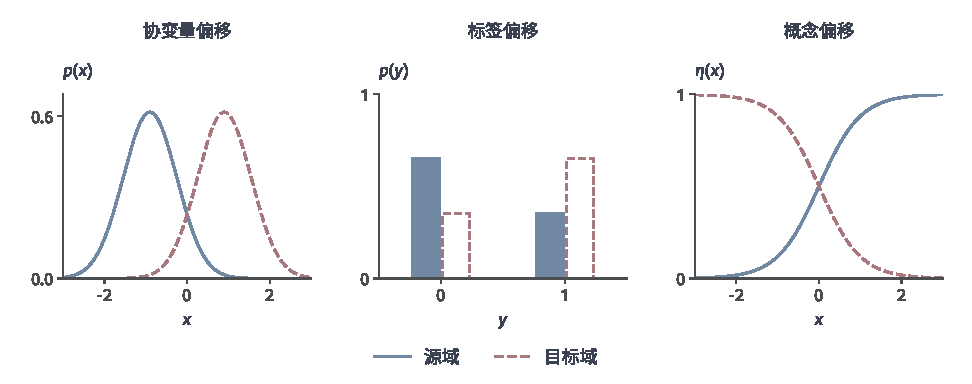
\includegraphics[width=164.600mm]{figures/06-foundations/02-learning-theory/matplotlib/learning-theory-distribution-shift/figure.pdf}
  \caption{分布偏移改变联合分布的不同组成部分。实线表示源域，虚线表示目标域；密度、类别比例和条件概率均为规范化的教学构造，不表示实测频率。协变量偏移允许输入分布改变，标签偏移允许类别比例改变，概念偏移则改变给定输入后的标签分布，图中$\eta(x)=\mathbb P(y=1\mid x)$。这些设定还需与覆盖条件或其他可识别条件结合，才能支持迁移保证。}
 \label{fig:learning-distribution-shift}
\end{figure*}

协变量偏移中条件标签规律不变，是否意味着三月学到的好规则在四月也好？对允许全部规则的候选空间是这样，对受限候选空间则未必。为单独观察输入比例的作用，暂把候选限制为恒预测0的$g_0$和恒预测1的$g_1$，采用零一损失；这个限制只为隔离比例的影响，不是推荐忽略邮件特征。$g_0$只在诈骗邮件上出错，按两种邮件的条件错误率求平均，三月风险为$0.9\times0.1+0.1\times0.9=0.18$，四月为$0.1\times0.1+0.9\times0.9=0.82$；$g_1$恰好相反。图~\ref{fig:lt9-proportion-swap-ranking}画出这一反转。三月的经验风险最小化随样本增多，会以趋于1的概率选择$g_0$，但它在四月的超额风险为$0.82-0.18=0.64$。增加三月样本只会把三月风险估计得更准，不会把三月的排序改成四月的排序。

\begin{figure}[htbp]
 \centering
 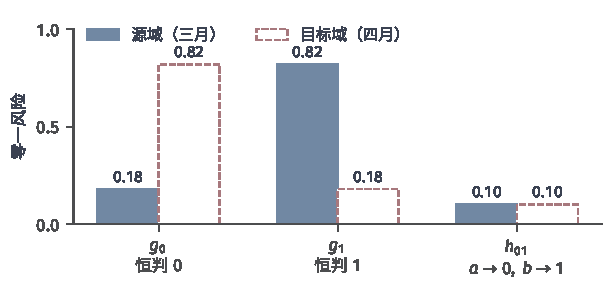
\includegraphics[width=104mm]{figures/06-foundations/02-learning-theory/matplotlib/lt9-proportion-swap-ranking/figure.pdf}
 \caption{两种邮件比例互换后候选的零一风险。实心柱为三月（$a,b$比例$0.9,0.1$），虚线空心柱为四月（比例$0.1,0.9$），两个月都有$\eta(a)=0.1$、$\eta(b)=0.9$。两个常值候选的排序在两个月相反；分别对$a,b$预测0、1的$h_{01}$是Bayes分类器，两个月风险都是0.10。}
 \label{fig:lt9-proportion-swap-ranking}
\end{figure}

图中第三个候选$h_{01}$在$a$上预测0、在$b$上预测1，它在两个月的风险都是$0.9\times0.1+0.1\times0.1=0.1\times0.1+0.9\times0.1=0.10$，始终最优。所以这个例子并不说明协变量偏移会改变Bayes决策；它说明的是，候选空间受限时，类内最优者可能随比例改变。实际模型总有表达限制，因此即使条件标签规律不变，也要直接分析目标风险，而不能只检查“预测规则有没有变”。

\subsubsection{可用观测与目标PAC要求}
\label{sec:transfer-pac-setting}

上面的例子只涉及一个分布对。要讨论“领域自适应能否学会”，需要像第~\ref{sec:pac-learning}节定义PAC可学习性那样，对一整族允许的情形提出统一要求。对同一个候选$h$，分别定义源域和目标域的总体风险
\begin{equation}
 R_D(h)=\mathbb E_{(x,y)\sim\mathcal P_D}\ell(h(x),y),
 \qquad D\in\{S,T\}.
 \label{eq:transfer-population-risks}
\end{equation}
目标域可能有标签噪声，候选空间也可能有表达限制，所以用$R_{T,\mathcal H}^{\star}=\inf_{h\in\mathcal H}R_T(h)$作比较基准，称$R_T(h)-R_{T,\mathcal H}^{\star}$为\term{目标域超额期望风险}（target-domain excess risk）。它衡量所选候选与同一候选空间中目标表现最好者的差距。

承接第~\ref{sec:transfer-feedback-information}节的反馈分档，本节以带标签源样本$S_S\sim\mathcal P_S^{n_S}$与无标签目标输入$U_T\sim(\mathcal P_T^X)^{n_T}$作为领域自适应的主要协议，两份样本相互独立。能否学习取决于允许的分布对集合$\mathfrak P_{\mathrm{DA}}$；覆盖关系、共享的标签规律都写进这个集合。若算法还需要已知的密度比等辅助知识，就把它列为算法的额外输入；若目标标签可用，那是另一种协议，不能把它得到的结论混入无监督结论。下面的定义沿用第~\ref{sec:pac-general-form}节的量词结构，只做两处改变：评价对象换成目标域超额风险，样本门槛分成源样本与目标样本两项。概率包含抽样与算法内部随机性。

\begin{definition}[领域自适应的PAC可学习性]
\label{def:adaptation-pac-learnability}
固定$\mathcal H,\ell,\mathfrak P_{\mathrm{DA}}$。若存在输出属于$\mathcal H$的算法$A$和有限门槛$m_S,m_T$，使对任意$\varepsilon,\delta\in(0,1)$、任意$(\mathcal P_S,\mathcal P_T)\in\mathfrak P_{\mathrm{DA}}$，以及$n_S\geq m_S(\varepsilon,\delta)$、$n_T\geq m_T(\varepsilon,\delta)$，都有
\[
 \mathbb P\{R_T(A(S_S,U_T))-R_{T,\mathcal H}^{\star}\leq\varepsilon\}
 \geq1-\delta,
\]
则称该设定PAC可学习。门槛可以依赖候选空间和分布族的统一参数，但不能依赖未知的具体分布对。
\end{definition}

这个要求与“某个模型在某个分布对上恰好正确”不同。对一个具体的分布对，总能挑出一个目标风险最小的候选；可学习性追问的是，同一个程序能否只凭规定的观测，在整个允许族上都选出它。门槛依赖哪些统一常数，例如权重上界或类别比例的下界，要在后面每条正面路线中写明。定义只要求有限样本下存在成功的算法，高效计算另需控制求解代价。
\subsubsection{相同观测下的不兼容目标决策}
\label{sec:transfer-incompatible-decisions}

有了统一要求，就能精确地说“源观测不足以学会”是什么意思。设两个月都以概率$1/2$产生输入0和1，三月的标签为$y=x$；四月的标签可能也是$y=x$，也可能变成$y=1-x$。在两种情形中，算法收到的带标签源样本与无标签目标输入有完全相同的分布，正确的目标决策却相反。图~\ref{fig:learning-alignment-counterexample}把同一个预测与两种隐藏标签并排比较。

\begin{figure*}[!htb]
  \centering
  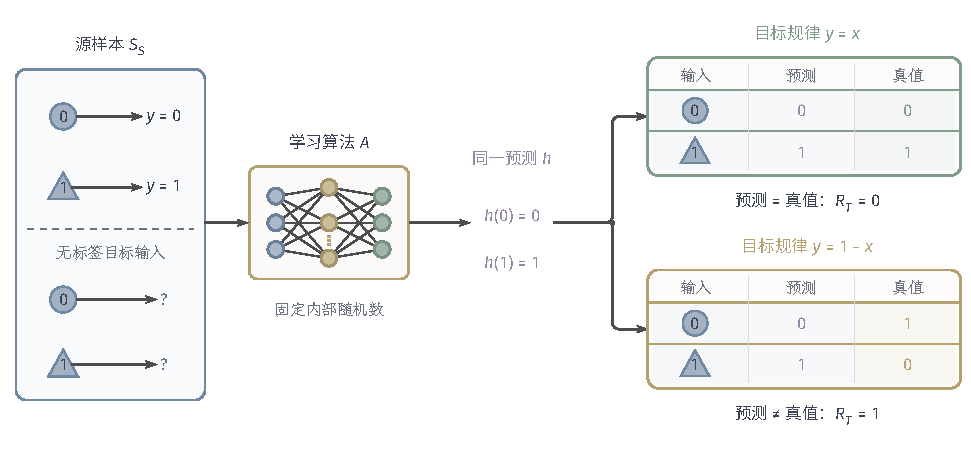
\includegraphics[width=164.600mm]{figures/06-foundations/02-learning-theory/tikz/learning-theory-alignment-counterexample/figure.pdf}
  \caption{相同可观察数据不能区分两种目标规律。两域都以概率$1/2$产生输入0或1，源标签为$y=x$。算法只收到左侧带标签源样本和无标签目标域训练样本，目标标签并未提供；右侧两种可能分别取$y=x$与$y=1-x$。固定算法内部随机数后，两种情形必得到同一训练分类器。图中以$h(x)=x$为例，两张表逐点对照同一预测与隐藏标签：零一损失下，源风险为0，两种目标风险分别为0、1。任意二分类器在这两种目标规律下的风险之和为1。输入完全对齐仍未提供选择目标规律的证据，还需目标标签或连接两域标签规律的额外条件。}
  \label{fig:learning-alignment-counterexample}
\end{figure*}

即使把两类样本都增加到无限多，可见信息也至多确定源联合分布和目标输入分布，算法仍然不知道目标标签属于哪种规律。于是问题不再是估计误差有多大，而是被估计的对象能否由这些信息确定。一个目标量是否由可观察数据的分布唯一确定，是\term{可识别性}（identifiability）问题。前几章没有遇到它，是因为训练样本与评价总体来自同一分布：样本无限多时，经验风险趋于总体风险，被估计的对象自然由数据确定。下面把反例写成定理。

\begin{theorem}[相同观测下的不可学习性]
\label{thm:transfer-nonidentifiability}
采用二分类零一损失。令$X=Y=\{0,1\}$，$\mathcal H$为$X$上全部四个二分类函数。源域$\mathcal P_S$令$x$在$\{0,1\}$上均匀、$y=x$；两个允许的目标域$\mathcal P_T^{+},\mathcal P_T^{-}$都令$x$均匀，分别取$y=x$与$y=1-x$。对任意$n_S,n_T\geq1$及任意只使用$S_S\sim\mathcal P_S^{n_S}$与独立的$U_T\sim(\mathcal P_T^X)^{n_T}$、输出属于$\mathcal H$的可能随机化算法$A$，总有一个目标域$\mathcal P_T\in\{\mathcal P_T^{+},\mathcal P_T^{-}\}$满足
\[
 \mathbb P\Bigl\{R_T(A(S_S,U_T))-R_{T,\mathcal H}^{\star}\geq\tfrac12\Bigr\}
 \geq\tfrac12 .
\]
两个目标域中都有$R_{T,\mathcal H}^{\star}=0$，概率包含抽样与算法内部随机性。
\end{theorem}
\begin{proof}
先看两个目标规律对同一个分类器$h$的评价。在每个输入上，$h(x)$恰好与$x$、$1-x$中的一个相等，所以$h$在两种目标规律下的逐点错误指示之和为1。对均匀的$x$取期望，得到
\[
 R_T^{+}(h)+R_T^{-}(h)=1\qquad\text{对每个}h\in\mathcal H.
\]
因此每个$h$至少在一个目标域上的风险不小于$1/2$。

再看算法的输出分布。两种情形中，$S_S$的分布相同，$U_T$只含目标输入，而两个目标域的输入分布都是均匀分布，所以$(S_S,U_T)$与算法内部随机数合在一起的联合分布完全相同，输出$\widehat h=A(S_S,U_T)$在两种情形中的分布也相同。记事件$E^{\pm}=\{R_T^{\pm}(\widehat h)\geq1/2\}$。由上一段，每个$\widehat h$都使$E^{+}$或$E^{-}$至少一个发生，故
\[
 \mathbb P(E^{+})+\mathbb P(E^{-})\geq1 ,
\]
其中两个概率按共同的输出分布计算。于是二者至少有一个不小于$1/2$。最后，$h(x)=x$与$h(x)=1-x$分别使两个目标风险为0，所以$R_{T,\mathcal H}^{\star}=0$，超额风险等于目标风险。
\end{proof}

定理把不可识别性落实到“近似最优的目标决策互不兼容”：只要求精度$\varepsilon<1/2$、失败概率$\delta<1/2$，任何算法都做不到。这比“两种目标的条件概率不同”更强，因为不同的条件概率可能拥有同一个最优决策。例如零一损失下，正类概率为0.7或0.8时都应预测1；两个目标域若只在这种意义上不同，算法不必区分它们也能作出好决策。所以，用不可识别性证明不可学习时，需要构造可见规律相同、而近似最优决策不兼容的两个来源，定理中的两种规律正是如此。

增加同一协议下的观测不会区分这两个来源，改变协议或允许族则会改变结论。提供少量四月标签后，两种规律在第一个带标签样本上就不同；规定允许族中的源、目标必须共享条件标签规律后，$y=1-x$与源规律不同，$\mathcal P_T^{-}$就被排除。反过来，识别好决策不要求恢复完整的目标分布：后面每条正面路线只需要一种足以确定目标风险排序的跨域联系，并须明确写出它是什么。

\subsection{领域自适应的风险保证}
\label{sec:adaptation-risk}

现在在“带标签源样本加无标签目标输入”的主要协议下，比较三条正面路线。协变量偏移保持条件标签规律，把目标风险精确改写为源分布上的按输入加权的期望；标签偏移保持类内输入规律，把目标风险改写为按类别加权的期望；预测分歧路线不要求精确改写，而是借助一个在两域都较好的参照候选，给出目标风险的上界。三条路线的假设和误差项不同，不能把其中一条的假设推广到全部迁移问题。

\subsubsection{协变量偏移下的重加权学习}
\label{sec:adaptation-coverage}

\paragraph{风险改写与覆盖条件}
先在有限输入上推导。记$r_h(x)=\mathbb E[\ell(h(x),y)\mid x]$为候选$h$在输入$x$处的条件损失。共享条件标签规律意味着$r_h(x)$在两域相同，于是
\[
 R_T(h)=\sum_x\mathcal P_T^X(x)\,r_h(x)
       =\sum_{x:\,\mathcal P_S^X(x)>0}\mathcal P_S^X(x)\,
        \frac{\mathcal P_T^X(x)}{\mathcal P_S^X(x)}\,r_h(x).
\]
第二个等号要求：凡是目标概率为正的输入，源概率也为正；否则这样的输入会从右侧求和中漏掉，而且比值的分母为零。满足这一要求时，目标风险就是源分布下的一个加权平均，每个输入的权重是它在目标域中的概率相对于源域的倍数。

一般输入空间中，相应条件是目标输入分布对源输入分布绝对连续，记作$\mathcal P_T^X\ll\mathcal P_S^X$：源域中概率为零的集合，在目标域中概率也为零。我们称之为源域覆盖目标域。这时Radon--Nikodym定理给出\term{密度比}（density ratio）$w=\mathrm d\mathcal P_T^X/\mathrm d\mathcal P_S^X$，离散情形就是$w(x)=\mathcal P_T^X(x)/\mathcal P_S^X(x)$。设两个域共享条件标签核$\mathsf K(\mathrm dy\mid x)$，则
\[
 \begin{aligned}
 R_T(h)
 &=\int_X\!\left[\int_Y\ell(h(x),y)\,\mathsf K(\mathrm dy\mid x)\right]
          \mathcal P_T^X(\mathrm dx)\\
 &=\int_X\!w(x)\left[\int_Y\ell(h(x),y)\,\mathsf K(\mathrm dy\mid x)\right]
          \mathcal P_S^X(\mathrm dx).
 \end{aligned}
\]
第一步先在同一输入上对标签取平均，第二步只替换输入积分所用的分布。共享条件标签核保证方括号中的计算可以继续使用源标签，覆盖保证这个替换存在。合写为源联合分布上的期望，得到
\begin{equation}
 R_T(h)=\mathbb E_{(x,y)\sim\mathcal P_S}[w(x)\ell(h(x),y)].
 \label{eq:covariate-risk-identity}
\end{equation}
这种按密度比给源损失加权的做法称为\term{重要性加权}（importance weighting）。条件概率核的存在与可测选取，可参考\BookChapterRef{chap:random-variables}{卷1《数学准备：基础数学》的“随机变量与概率分布”章}。绝对连续性只负责风险能够改写；要从有限样本估计右侧，还需要权重的统一上界或适当的矩条件，这一步下面另外承担。

覆盖只排除完全没有源观测的区域，并不保证目标常见的输入在源域也常见。图~\ref{fig:learning-support-coverage}显示覆盖与密度相同是两种要求：源、目标密度可以不同，缺少覆盖的区域却无法仅靠更多源观测补出标签。

\begin{figure*}[!htb]
  \centering
  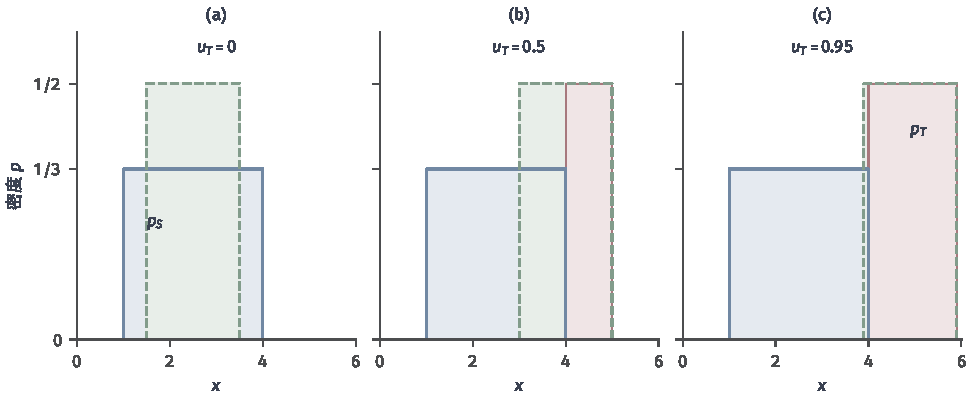
\includegraphics[width=164.600mm]{figures/06-foundations/02-learning-theory/matplotlib/learning-theory-support-coverage/figure.pdf}
  \caption{同尺度的三种支持覆盖。源密度均为$[1,4]$上的$1/3$，目标密度均为长度2区间上的$1/2$；(a)、(b)、(c)的目标支持依次为$[1.5,3.5]$、$[3,5]$、$[3.9,5.9]$。深色区域没有源密度，其目标概率$u_T=\mathbb P_T\{p_S(X)=0\}$依次为0、0.5、0.95。实线、虚线与底色共同区分源域、目标域；只有(a)满足覆盖条件$p_T(x)>0\Rightarrow p_S(x)>0$。密度为规范化教学构造，不是实验分布。}
 \label{fig:learning-support-coverage}
\end{figure*}
\paragraph{没有覆盖时的不可学习性}
覆盖条件为什么不能省？设源域从不出现促销邮件$b$，四月却全是$b$。“共享条件标签规律”只约束两域都有可能出现的输入；在$b$处，源域没有任何观测，这个假设也就不提供任何约束。图~\ref{fig:lt9-coverage-gap}把这个缺口画成两个可能的世界：两种世界中，算法收到的数据都是“源样本全为$(a,0)$、目标输入全为$b$”，而$b$的目标标签一个为0、一个为1。

\begin{figure}[htbp]
 \centering
 % 第9章：源域看不到目标输入的覆盖缺口（定理 thm:covariate-coverage-failure 的构造）。
% X={a,b}；源域恒产生 (a,0)，目标输入恒为 b；b 的目标标签恒为 0 或恒为 1。
% 候选 h_0(a)=h_1(a)=0，h_0(b)=0，h_1(b)=1。零一损失下目标风险：
% b 标签为 0 时 R_T(h_0)=0、R_T(h_1)=1；b 标签为 1 时 R_T(h_0)=1、R_T(h_1)=0。
\begingroup
\definecolor{FigureGreen}{HTML}{829C8B}
\definecolor{FigureGreenFill}{HTML}{E8EEE9}
\begin{tikzpicture}[figure picture,x=1mm,y=1mm]
% 左：两个输入上的概率；每行左侧为行名
\node[figure note,anchor=east] at (12,27) {源域};
\node[figure note,anchor=east] at (12,7) {目标域};
\draw[FigureStroke,line width=.6pt] (14,22) -- (48,22);
\draw[FigureStroke,line width=.6pt] (14,2) -- (48,2);
\fill[FigureBlueFill,draw=FigureBlue] (19,22) rectangle (27,34);
\node[figure note,align=center] at (23,28) {概率1\\标签0};
\draw[FigureRed,line width=.6pt,dash pattern=on 2pt off 1.5pt] (36,22) rectangle (44,34);
\node[figure note,text=FigureRed,align=center] at (40,28) {概率0};
\node[font=\figurefont\footnotesize] at (23,19.8) {$a$};
\node[font=\figurefont\footnotesize] at (40,19.8) {$b$};
\fill[FigureRedFill,draw=FigureRed] (36,2) rectangle (44,14);
\node[figure note,align=center] at (40,8) {概率1\\标签?};
\node[font=\figurefont\footnotesize] at (23,-0.2) {$a$};
\node[font=\figurefont\footnotesize] at (40,-0.2) {$b$};
% 右：两个候选在两个可能世界中的目标风险
\begin{scope}[shift={(56,0)}]
\node[figure heading,anchor=west] at (0,37) {两个候选与两个可能目标};
\foreach \x/\w/\t in {0/10/{},10/9/{$h(a)$},19/9/{$h(b)$},28/13/{$b$标0},41/13/{$b$标1}}{%
  \node[draw=FigureGrid,minimum width=\w mm,minimum height=6.4mm,inner sep=0pt,
    anchor=north west,font=\figurefont\footnotesize] at (\x,32) {\t};}
\foreach \y/\h/\pa/\pb/\ra/\rb/\fa/\fb in {25.6/$h_0$/0/0/0/1/FigureGreenFill/FigureRedFill,
                                           19.2/$h_1$/0/1/1/0/FigureRedFill/FigureGreenFill}{%
  \node[draw=FigureGrid,minimum width=10mm,minimum height=6.4mm,inner sep=0pt,anchor=north west,font=\figurefont\footnotesize] at (0,\y) {\h};
  \node[draw=FigureGrid,minimum width=9mm,minimum height=6.4mm,inner sep=0pt,anchor=north west,font=\figurefont\footnotesize] at (10,\y) {\pa};
  \node[draw=FigureGrid,minimum width=9mm,minimum height=6.4mm,inner sep=0pt,anchor=north west,font=\figurefont\footnotesize] at (19,\y) {\pb};
  \node[draw=FigureGrid,fill=\fa,minimum width=13mm,minimum height=6.4mm,inner sep=0pt,anchor=north west,font=\figurefont\footnotesize] at (28,\y) {\ra};
  \node[draw=FigureGrid,fill=\fb,minimum width=13mm,minimum height=6.4mm,inner sep=0pt,anchor=north west,font=\figurefont\footnotesize] at (41,\y) {\rb};}
\node[figure note,anchor=north west,align=left] at (0,11) {后两列为目标风险 $R_T(h)$。两种世界中\\算法收到的数据都是“全为 $(a,0)$，全为 $b$”。};
\end{scope}
\end{tikzpicture}
\endgroup

 \caption{源域看不到目标输入造成的覆盖缺口。左图上行为源域输入概率：源域只产生标签为0的$a$，在$b$上概率为0（虚线框）；下行为目标域，只产生标签未知的$b$。右表列出两个候选在$a,b$上的预测，以及它们在“$b$标0”“$b$标1”两种世界中的目标零一风险；绿格为0，红格为1。两种世界给出同一份观测，每种世界又各有一个候选在两域都零风险。}
 \label{fig:lt9-coverage-gap}
\end{figure}

\begin{theorem}[缺少覆盖时的不可学习性]
\label{thm:covariate-coverage-failure}
采用二分类零一损失。令$X=\{a,b\}$、$Y=\{0,1\}$，且$\mathcal H=\{h_0,h_1\}$满足
\[
 h_0(a)=h_1(a)=0,\qquad h_0(b)=0,\quad h_1(b)=1.
\]
源域分布$\mathcal P_S$恒产生$(a,0)$，目标域输入边缘分布恒产生$b$；允许的两个目标域分布分别令$b$的标签恒为0或恒为1。对任意$n_S,n_T\geq1$，令$S_S\sim\mathcal P_S^{n_S}$与$U_T\sim(\mathcal P_T^X)^{n_T}$相互独立。对任意只使用这两份样本、输出属于$\mathcal H$的可能随机化学习算法$A$，总有一个允许的目标域满足
\[
 \mathbb P\bigl\{R_T(A(S_S,U_T))>\tfrac14\bigr\}\geq\tfrac12 .
\]
概率包含抽样与算法内部随机性。两个设定中都各有一个候选的源域与目标域风险同时为零。
\end{theorem}
\begin{proof}
两种设定中，算法收到的源样本都是$n_S$个$(a,0)$，目标输入都是$n_T$个$b$，因此输入数据完全相同。设算法输出$h_1$的概率为$p$；这个概率只来自算法内部随机性，在两个设定中相同。目标标签为0时，算法以概率$p$输出$h_1$，其目标零一风险为1；目标标签为1时，算法以概率$1-p$输出$h_0$，其目标零一风险也为1。$p$与$1-p$至少有一个不小于$1/2$。标签为0的设定中$h_0$在两域都无错误，标签为1的设定中$h_1$在两域都无错误，所以失败并非候选空间缺少合适的候选。
\end{proof}

无论样本量多大，$b$的标签都没有进入观测。这里甚至存在同时在源域和目标域零风险的候选，所以“存在一个两域都好的模型”不能代替“从观测中识别出它”。与定理~\ref{thm:transfer-nonidentifiability}相比，这里两个世界在源域可见的输入上标签规律完全一致，失败只来自覆盖缺口。这个障碍针对所构造的允许族：$\mathcal H$中的候选在$a$上一致、在$b$上任意，$a$的观测对$b$毫无约束。若候选结构把$a$与$b$的标签联系起来，例如只允许在两点上预测相同类别，那么$a$处的观测就约束了$b$，问题需要重新分析。所以不能断言任何迁移问题都必须满足同一种覆盖条件；它是重加权路线所需的条件，也是这一类缺少结构联系的问题的障碍\scite{bendavid2010impossibility}。

\paragraph{重加权改变候选排序}
回到三月、四月两种邮件的例子。密度比为$w(a)=0.1/0.9=1/9$、$w(b)=0.9/0.1=9$。设一次教学构造的三月样本含100封邮件：90封为$a$，其中9封是诈骗；10封为$b$，其中9封是诈骗。未加权时，$g_0$错在18封诈骗邮件上，$g_1$错在82封正常邮件上，源经验最优者是$g_0$。加权以后，每封$a$只计$1/9$，每封$b$计9，经验风险变为
\[
 \begin{aligned}
 \widehat R_w(g_0)&=\frac{9\times\frac19+9\times9}{100}=0.82,\\
 \widehat R_w(g_1)&=\frac{81\times\frac19+1\times9}{100}=0.18.
 \end{aligned}
\]
同一批标签没有改变，少见的$b$邮件却按它在四月的分量计分，选择因而转为$g_1$。图~\ref{fig:lt9-reweighting-ranking}把每个候选的错误按来源拆开：未加权时$g_1$的错误几乎都来自$a$，加权后$a$的贡献缩小为原来的$1/9$，$b$的贡献放大9倍。这些经验值恰好等于前面的目标风险，是构造计数的结果；一般样本仍有波动。图~\ref{fig:learning-importance-weighting}在连续输入上展示同一种概率重分配。

\begin{figure}[htbp]
 \centering
 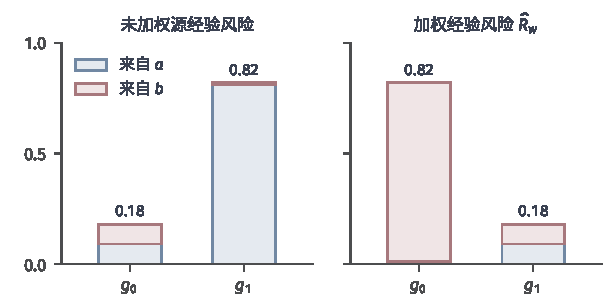
\includegraphics[width=104mm]{figures/06-foundations/02-learning-theory/matplotlib/lt9-reweighting-ranking/figure.pdf}
 \caption{重加权前后两个常值候选的经验风险。教学样本为90封$a$（9封诈骗）与10封$b$（9封诈骗）；每段高度为该来源的错误数乘以权重再除以100，左图权重为1，右图取$w(a)=1/9$、$w(b)=9$。左图源经验最优者为$g_0$，右图为$g_1$，与四月的目标风险排序一致。}
 \label{fig:lt9-reweighting-ranking}
\end{figure}

\begin{figure}[htbp]
  \centering
  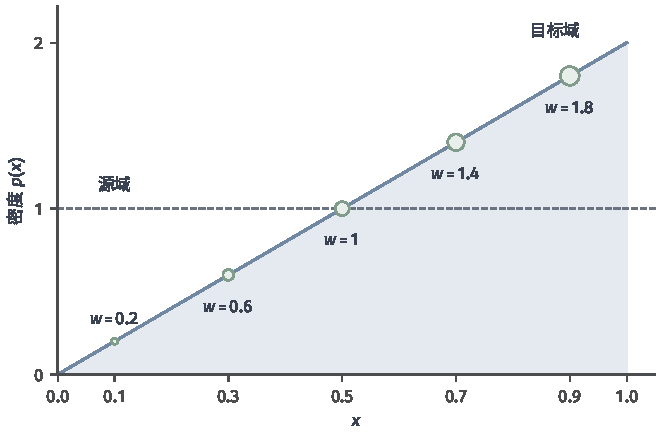
\includegraphics[width=112.000mm]{figures/06-foundations/02-learning-theory/matplotlib/learning-theory-importance-weighting/figure.pdf}
  \caption{重要性权重重新分配源样本的贡献。在$[0,1]$上构造源密度$p_S(x)=1$、目标密度$p_T(x)=2x$，二者均积分为1，因此$w(x)=2x$。五个源样本位置人为取为0.1、0.3、0.5、0.7、0.9，权重依次为0.2、0.6、1、1.4、1.8。圆点叠在目标密度上，面积与权重成正比，面积不表示局部样本数量。目标输入必须受到源输入覆盖；要使用风险恒等式，还需保持相同的条件标签分布。}
 \label{fig:learning-importance-weighting}
\end{figure}

\paragraph{已知有界权重的有限样本保证}
大权重也会放大有限样本的波动。若把三月中$b$的比例从0.1减为很小的$u>0$，四月仍以0.9的概率产生$b$，那么$w(b)=0.9/u$。$n$个源样本完全没有$b$的概率为$(1-u)^n$；即使看见一个，它的贡献也可能很大。覆盖只要求$u>0$，并没有排除少量源观测承担大量目标概率的情形。为了得到对允许族统一的有限样本界，以下假定$w$已知且$0\leq w\leq\kappa$，这个上界限制目标区域相对于源域能有多常见。设$\mathcal H$含$N$个可测候选，对$n$个独立源样本计算
$\widehat R_w(h)=n^{-1}\sum_{i=1}^n w(x_i)\ell(h(x_i),y_i)$，并选取其近似最小者。

\begin{theorem}[已知密度比下的迁移样本量界]
\label{thm:covariate-finite-pac}
在共享条件标签核、覆盖、已知密度比$0\leq w\leq\kappa$及有限候选空间条件下，若算法输出满足
$\widehat R_w(\widehat h)\leq\min_{h\in\mathcal H}\widehat R_w(h)+\rho$，其中$\rho\geq0$，则以概率至少$1-\delta$，
\begin{equation}
 R_T(\widehat h)-R_{T,\mathcal H}^{\star}
 \leq\kappa\sqrt{\frac{2\log(2N/\delta)}{n}}+\rho.
 \label{eq:covariate-finite-excess}
\end{equation}
\end{theorem}
\begin{proof}
由式~\eqref{eq:covariate-risk-identity}，每个加权损失的均值就是待估计的目标风险；由权重上界，加权损失取值在$[0,\kappa]$中。对任意固定候选，Hoeffding不等式给出偏差超过$a$的概率至多为$2\exp(-2na^2/\kappa^2)$。对$N$个候选求和，得到概率至少为$1-\delta$的同一个事件，在该事件上
\[
 \sup_{h\in\mathcal H}|\widehat R_w(h)-R_T(h)|
 \leq a_n=\kappa\sqrt{\frac{\log(2N/\delta)}{2n}}.
\]
这个偏差事件对全部候选同时成立，可以用于由数据选出的$\widehat h$；只对预先固定的单个候选成立的估计不够。取目标风险最小者$h^\star$，在这个事件上应用定理~\ref{thm:approximate-erm-risk}的三步比较，其中经验风险换成加权经验风险、总体风险换成目标风险：
\[
 R_T(\widehat h)\leq\widehat R_w(\widehat h)+a_n
 \leq\widehat R_w(h^\star)+\rho+a_n
 \leq R_T(h^\star)+\rho+2a_n .
\]
$2a_n$化简即得式中的根号项。
\end{proof}

候选的损失可以计算、候选间可以比较时，精确枚举可令$\rho=0$，此时$n\geq2\kappa^2\log(2N/\delta)/\varepsilon^2$足以保证超额风险不超过$\varepsilon$；若只能做到$\rho\leq\varepsilon/2$，就把抽样项也控制到$\varepsilon/2$。模型选择的可行性由此拆成可以分别检验的两项：样本能否区分目标风险，求解过程能否找到足够小的加权经验风险。

这里的$\kappa^2$来自按取值范围估计的Hoeffding界，是充分条件中的代价，不是普遍最优的下界。对固定候选，令$Z=w(x)\ell(h(x),y)$，独立抽样给出$\operatorname{Var}(\widehat R_w(h))=\operatorname{Var}_S(Z)/n$；又因为$\mathbb E_Sw=1$且$w^2\leq\kappa w$，有$\operatorname{Var}_S(Z)\leq\mathbb E_Sw^2\leq\kappa$。利用方差信息可以得到比仅按取值范围更细的界，但它仍取决于目标概率是否集中在源域稀少的输入上。两种邮件的例子中，$\mathbb E_Sw^2=0.9\times(1/9)^2+0.1\times9^2=73/9\approx8.1$，而分布不变时这个量为1。若枚举候选过于昂贵，还要另行分析优化算法；有限样本保证不是高效计算保证。
\paragraph{无限候选：复杂度与稳定性}
\label{sec:transfer-stability}
上面的证明对$N$个候选的失败概率求和，样本量界中出现$\log N$；候选无穷多时这一项失去意义。第~\ref{sec:rademacher-complexity}节用衡量函数族拟合能力的复杂度代替候选个数，这里可以照搬，唯一的改动是：要控制的对象是\emph{加权后}的损失函数族，因为权重会放大某些样本的影响。独立源样本上的经验Rademacher复杂度为
\[
 \widehat{\mathfrak R}_S(w\ell_{\mathcal H})
 =\mathbb E_{\bm\sigma}\sup_{h\in\mathcal H}
 \frac1n\sum_{i=1}^n\sigma_i w(x_i)\ell(h(x_i),y_i),
\]
其中$\sigma_i$独立、等概率取$\pm1$。沿用那里的对称化与有界差分分析，加权损失取值于$[0,\kappa]$，以概率至少$1-\delta$，
\[
 \sup_h|R_T(h)-\widehat R_w(h)|
 \leq2\widehat{\mathfrak R}_S(w\ell_{\mathcal H})
      +3\kappa\sqrt{\frac{\log(4/\delta)}{2n}}.
\]
这里合并了正、负两个方向的偏差事件，并假定相应上确界可测。近似ERM的目标超额风险由右侧的两倍加优化误差控制，跨域联系仍由式~\eqref{eq:covariate-risk-identity}提供。

另一条路径不考察整个函数族，而是沿用第~\ref{sec:algorithmic-stability}节的算法稳定性：替换一个训练样本几乎不改变输出的算法，经验风险与总体风险之差在期望上也小。设替换一个源样本后，实际运行的\emph{加权}算法的输出在任意观测上的期望未加权损失变化至多为$\beta_n$，且其期望加权经验优化误差至多为$\rho_n$。乘上固定权重后，加权损失的敏感度至多为$\kappa\beta_n$。由于目标风险等于加权源风险，定理~\ref{thm:stability-expected-generalization}与定理~\ref{thm:expected-risk-comparison}的期望比较给出
\begin{equation}
 \mathbb E\big[R_T(A(S))-R_{T,\mathcal H}^{\star}\big]
 \leq\kappa\beta_n+\rho_n.
 \label{eq:transfer-stability-excess}
\end{equation}
其依据是把超额风险分成期望泛化差与经验优化差，再用$\mathbb E\inf_h\widehat R_w(h)\leq\inf_hR_T(h)$处理比较基准。若右侧在允许族上一致趋零，非负超额风险的Markov不等式便把期望界转为PAC保证。注意$\beta_n$必须针对实际运行的加权算法验证：同一个算法在未加权数据上稳定，并不说明它在权重最大可达$\kappa$的数据上同样稳定。

复杂度与稳定性提供不同的有限样本控制方式，但都没有创造跨域标签联系。用PAC--Bayes分析随机预测器时也一样：源样本选择参数分布的代价可以控制，目标标签机制仍需单独建立依据。这些工具接在可识别条件之后使用，不能把一个随样本量减小的估计项当作完整的迁移结论。

\paragraph{权重未知时的估计}
已知$w$的结论没有用到无标签目标样本，因为分布差异已经由辅助输入提供。$w$未知时，目标样本的作用是帮助估计它。设从独立的辅助数据得到$0\leq\widehat w\leq\kappa$，并以概率至少$1-\delta_w$满足
$\mathbb E_{x\sim\mathcal P_S^X}|\widehat w(x)-w(x)|\leq b_w$。由于损失不超过1，对全部候选都有
\[
 \left|\mathbb E_S[\widehat w(x)\ell(h(x),y)]-R_T(h)\right|
 \leq\mathbb E_S|\widehat w-w|\leq b_w .
\]
条件于辅助数据，$\widehat w$是一个固定的有界函数，对新的独立源标签样本使用上一证明即可控制它的经验均值。算法用这些样本近似最小化$\widehat R_{\widehat w}$，经验优化误差至多为$\rho$。所选候选与目标最优的比较候选各付一次权重误差，所以以概率至少$1-\delta_w-\delta_\ell$，
\[
 R_T(\widehat h)-R_{T,\mathcal H}^{\star}
 \leq\kappa\sqrt{\frac{2\log(2N/\delta_\ell)}{n_\ell}}+2b_w+\rho .
\]
这里$n_\ell$是用于损失估计的独立源样本数；若另用$m_S$个源输入估计权重，源样本总数为$n_S=n_\ell+m_S$。独立划分是展示这条证明的一种充分安排；用同一批数据既估计权重又估计损失时，权重依赖于这批样本，需要对权重的可能取值另作统一控制。

仍看两种邮件的例子，先假定三月比例已知，四月中$b$的比例$q=\mathcal P_T^X(b)$未知。用$n_T$个无标签四月输入中$b$的频率$\widehat q$估计它，再令$\widehat w(b)=\widehat q/0.1$、$\widehat w(a)=(1-\widehat q)/0.9$。未截断的估计满足
\[
 \mathbb E_S|\widehat w-w|
 =0.1\cdot\frac{|\widehat q-q|}{0.1}+0.9\cdot\frac{|\widehat q-q|}{0.9}
 =2|\widehat q-q| .
\]
若将估计逐点截到已知的$[0,\kappa]$，由于真权重也在其中，左侧只会减小。由Hoeffding不等式，可取$b_w=2\sqrt{\log(2/\delta_w)/(2n_T)}$，使所需事件以概率至少$1-\delta_w$成立。这时目标样本只回答“$b$邮件有多常见”，诈骗概率仍由源标签和共享条件核提供；增加目标输入不能替代源标签。

若三月比例也未知，密度比的估计还要除以源频率。源概率很小的输入可能在辅助样本中一次也未出现，或者使分母的误差被放大。因此这个有限输入例子需要源概率的统一正下界，或其他能稳定估计所需比值的条件，才能把辅助源样本数也变成统一门槛。对一般输入空间，候选有限并不保证任意密度比都能可靠估计；沿这条路线证明PAC可学习，必须同时使加权损失误差、权重误差和优化误差在允许族上一致减小。

\paragraph{截断权重与近似共享的标签规律}
为了减小大权重的波动，可以把已知的$w$截到$0\leq\tau<\kappa$，即改用$\min\{w,\tau\}$。截断也改变了所估计的总体期望：被削去的权重可能恰好属于目标常见的区域。损失属于$[0,1]$时，每个候选的风险偏差至多为$\mathbb E_S[(w-\tau)_+]$，其中$(v)_+=\max\{v,0\}$；超额风险界的抽样项随$\tau$缩小，另加两倍的这项偏差。两种邮件的例子中取$\tau=3$，偏差上界为$0.1\times(9-3)=0.6$，这时界已不足以区分两个常值候选。截断需要同时衡量抽样波动和这项偏差，不能在定理~\ref{thm:covariate-finite-pac}中直接把$\kappa$换小而保留其余结论。

共享条件标签核也承担着不可省略的作用。若它仅近似成立，记两域的条件标签核为$\mathsf K_S,\mathsf K_T$，并令
$b_{\mathrm{cond}}=\mathbb E_{x\sim\mathcal P_T^X}d_{\mathrm{TV}}(\mathsf K_S(\cdot\mid x),\mathsf K_T(\cdot\mid x))$，即在目标输入分布下平均比较同一输入处的两种标签分布。总变差距离控制$[0,1]$值函数期望之差，因而每个候选的目标风险与加权源风险相差至多$b_{\mathrm{cond}}$，超额风险上界再增加$2b_{\mathrm{cond}}$。目标标签不可见时，这项偏差不能靠更精确地估计输入比例来消除。截断偏差与标签关系误差都是固定残余：它们限制当前上界能证明的精度，却不自动构成不可学习的下界。

\subsubsection{标签偏移下的类别重加权}
\label{sec:adaptation-label-shift}

\paragraph{类别加权的风险表示}
标签偏移改为保持各类别内部的输入分布、允许类别比例改变。记类别$y$的类内输入分布为$\mathsf K_y=\mathcal P(\cdot\mid y)$，在两域相同；记目标类别比例为$q_y=\mathcal P_T^Y(y)$，并设源域各类别的概率$\pi_y=\mathcal P_S^Y(y)$均为正。由于类内分布不变，变化只发生在类别比例上，权重应按类别而不是按输入分配：
\begin{equation}
 R_T(h)=\sum_y q_y\,\mathbb E_{x\sim\mathsf K_y}\ell(h(x),y)
       =\mathbb E_{(x,y)\sim\mathcal P_S}\Bigl[\frac{q_y}{\pi_y}\,\ell(h(x),y)\Bigr].
 \label{eq:label-shift-risk-identity}
\end{equation}
第一个等号按目标的第二种分解展开风险，第二个等号把每个类别的期望换回源分布，并以$\pi_y$除去源类别比例。这个假设不要求输入给定后的标签概率保持不变。

用一个新的两邮件构造检查这一点：令$\mathsf K_1(b)=0.8$、$\mathsf K_0(b)=0.2$，三月诈骗比例$\pi_1=0.5$，四月为$q_1=0.1$。三月看到$b$时诈骗的概率为$0.5\times0.8/(0.5\times0.8+0.5\times0.2)=0.8$，四月则为$0.1\times0.8/(0.1\times0.8+0.9\times0.2)=0.08/0.26\approx0.31$。同一种邮件的条件诈骗概率改变了，所以这不是协变量偏移。零一损失下，三月的Bayes决策在$b$上判1、在$a$上判0，风险为$0.5\times0.2+0.5\times0.2=0.2$；四月中这个决策的风险为$0.1\times0.2+0.9\times0.2=0.2$，而恒判0的风险只有$q_1=0.1$。按式~\eqref{eq:label-shift-risk-identity}取权重$q_1/\pi_1=0.2$、$q_0/\pi_0=1.8$，在三月数据上计算恒判0的加权风险为$0.2\times0.5=0.1$，计算三月Bayes决策的加权风险为$0.2\times0.5\times0.2+1.8\times0.5\times0.2=0.2$。加权源风险与目标风险逐一相等，排序随之改变。
\paragraph{从目标输入反解类别比例}
困难在于目标标签不可见，$q_y$不能直接计数。可利用的线索是目标输入：各类别内部的输入规律不变，所以目标输入分布就是这些类内分布按目标比例的混合，
\begin{equation}
 \mathcal P_T^X=\sum_y q_y\,\mathsf K_y .
 \label{eq:label-shift-mixture}
\end{equation}
类内分布可以由带标签源样本估计，目标输入分布可以由无标签目标样本估计，于是可以反解混合比例。在上面的构造中，$\mathcal P_T^X(b)=0.8q_1+0.2(1-q_1)=0.2+0.6q_1$；四月观测到$\mathcal P_T^X(b)=0.26$，便得到$q_1=(0.26-0.2)/0.6=0.1$。

这里要分开两个问题。第一个是\emph{识别}：混合分解是否唯一。若两个类内比例相同，例如$\mathsf K_0(b)=\mathsf K_1(b)=0.5$，目标输入就不再随$q_1$变化，任何$q_1$都与观测相容。一般有限类别下，类内分布$\{\mathsf K_y\}$线性无关可保证式~\eqref{eq:label-shift-mixture}中比例的唯一性。第二个是\emph{估计}：识别成立后，有限样本误差会被放大多少。二分类且类内分布已知时，
\[
 |\widehat q_1-q_1|=\frac{|\widehat{\mathcal P}_T^X(b)-\mathcal P_T^X(b)|}{|\mathsf K_1(b)-\mathsf K_0(b)|},
\]
分母越小，同样的输入频率误差反解出的比例误差越大。图~\ref{fig:lt9-label-shift-mixture}画出三组类内比例：观测带宽为$\pm0.03$时，差为0.6的情形把$q_1$限制在长0.1的区间内，差为0.1的情形只能限制到长0.6的区间，差为0的情形完全无法限制。统一的有限样本门槛因此需要类内分布的定量分离，例如二分类时$|\mathsf K_1(b)-\mathsf K_0(b)|$有统一下界，或多分类时相应矩阵的最小奇异值有统一下界。

\begin{figure}[htbp]
 \centering
 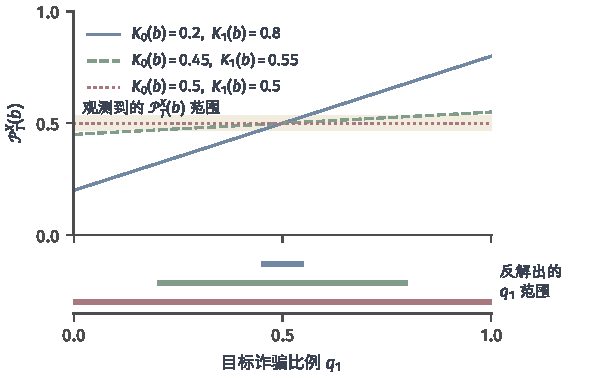
\includegraphics[width=104mm]{figures/06-foundations/02-learning-theory/matplotlib/lt9-label-shift-mixture/figure.pdf}
 \caption{标签偏移下目标输入分布是类内分布的混合，$\mathcal P_T^X(b)=\mathsf K_0(b)+[\mathsf K_1(b)-\mathsf K_0(b)]q_1$。三条线对应三组类内比例，黄色带为观测到的$\mathcal P_T^X(b)\in[0.47,0.53]$。下方横条是与观测带相容的$q_1$范围：类内比例相差0.6、0.1、0时，范围依次为$[0.45,0.55]$、$[0.2,0.8]$、$[0,1]$。直线越平，同样的输入误差反解出的比例误差越大。}
 \label{fig:lt9-label-shift-mixture}
\end{figure}

\paragraph{比例估计与目标风险}
有了比例估计，就可以沿用协变量偏移中已建立的加权经验风险比较。按类别加权时，权重误差为
\[
 \mathbb E_S|\widehat w(y)-w(y)|=\sum_y\pi_y\Bigl|\frac{\widehat q_y}{\pi_y}-\frac{q_y}{\pi_y}\Bigr|
 =\sum_y|\widehat q_y-q_y| ,
\]
其中先假定源类别比例$\pi_y$已知；二分类时它等于$2|\widehat q_1-q_1|$。权重上界为$\kappa=\max_yq_y/\pi_y\leq1/\min_y\pi_y$。把这两项代入上一小节“权重未知”的结论，就得到目标超额风险界：抽样项$\kappa\sqrt{2\log(2N/\delta_\ell)/n_\ell}$，加两倍的权重误差和优化误差。在二分类、类内分布已知的情形中，由Hoeffding不等式，以概率至少$1-\delta_w$，
\[
 2|\widehat q_1-q_1|\leq\frac{2}{|\mathsf K_1(b)-\mathsf K_0(b)|}\sqrt{\frac{\log(2/\delta_w)}{2n_T}} ,
\]
这就是目标输入需要承担的部分；源标签则一方面用于计算加权损失，另一方面在类内分布未知时用于估计$\mathsf K_y$。估计$\mathsf K_y$时，类别$y$只有约$\pi_yn_S$个源样本可用；若某个类别的源概率可以任意趋近零，固定数量的源样本可能完全看不到它。所以沿这条路径给出统一门槛，还需要源类别概率的统一下界，或能提供相应类内信息的其他条件。实践中常用一个已训练的分类器代替原始输入，用它在源样本上的混淆矩阵与在目标输入上的预测频率反解比例；可逆性条件变成该混淆矩阵可逆\scite{ket-lipton2018-labelshift}。

这条路线只继承了加权损失的统计论证。比例的识别依赖类内分布不变与线性无关，与协变量偏移中密度比的存在和估计是两套不同的条件，二者不能互相替代：图~\ref{fig:lt9-joint-factorizations}中的协变量偏移改变了类内分布，类别加权在那里不能改写目标风险；本小节的标签偏移改变了$\eta$，按输入加权在这里也不能。

\subsubsection{预测分歧与跨域风险界}
\label{sec:adaptation-divergence}

前两条路线都要求某个因子完全不变，并把目标风险精确改写为源期望。第三条路线放弃精确改写，只求一个上界：已有候选在源域错误较少时，能否借助可观察的输入差异，再加上一项刻画标签联系的量，限制它在目标域的错误？

\paragraph{分歧散度与风险界}
关键在于找一个与目标错误有关、又不需要目标标签就能计算的量。两个二分类器$h,g$在哪些输入上给出不同预测，只取决于输入，所以它们的分歧概率可以在无标签目标样本上直接估计。分歧又与错误相关：若$h$在某个输入上出错而$g$答对，二者必然分歧。于是，只要找到一个在目标域错误少的参照候选$g$，$h$的目标错误就不超过$g$的目标错误加上二者的目标分歧。剩下的困难是，$g$与$h$的目标分歧还要和源域上的量联系起来，这需要比较同一对分类器在两域中的分歧概率差多少。对二分类零一损失，令
\begin{equation}
 d_{\mathcal H\triangle\mathcal H}
 =2\sup_{h,g\in\mathcal H}
 \left|\mathbb P_S^X(h\neq g)-\mathbb P_T^X(h\neq g)\right| ,
 \label{eq:h-delta-h-divergence}
\end{equation}
其中$\mathbb P_D^X(h\neq g)$是在域$D$的输入分布下二者分歧的概率。这个量称为$\mathcal H\triangle\mathcal H$散度（$\mathcal H\triangle\mathcal H$-divergence），记号中的$\mathcal H\triangle\mathcal H$指全部分歧区域$\{x:h(x)\neq g(x)\}$构成的集合族。两种邮件的例子中，一对只在$b$上分歧的候选，其分歧概率在三月和四月分别为0.1和0.9；两者之差说明源域对这类预测差异赋予的权重与目标域不同。取上确界，是因为$h$由数据选出、参照候选$g$又未知，必须对所有可能的候选对同时控制；系数2采用文献中的惯用归一化。它只比较$\mathcal H$能够表达的分歧区域上的概率，而不是两个输入分布的全部差别。

散度只处理“输入在两域出现得是否一样频繁”，还没有涉及真实标签。前面的论证需要一个在目标域错误少的参照候选，又要用它在源域的错误把分歧转回源风险，因此它最好在两域都较少出错。定义
\[
 \lambda=\inf_{g\in\mathcal H}\bigl(R_S(g)+R_T(g)\bigr).
\]
它衡量\emph{同一个}候选在两域上能达到多小的风险之和，刻画两域的标签规律能否被同一个候选同时拟合；分别在两个域各找一个好候选，并不能使它变小。由于$\lambda$涉及目标风险，它无法由无标签目标样本估计，只能由对问题的假设来保证。

\begin{theorem}[领域自适应的目标域期望风险界]
\label{thm:domain-adaptation-bound}
对非空可测二分类候选空间$\mathcal H$和源、目标联合分布，采用零一损失及上述分歧散度与$\lambda$，则每个$h\in\mathcal H$都满足
\begin{equation}
 R_T(h)\leq R_S(h)+\tfrac12d_{\mathcal H\triangle\mathcal H}+\lambda.
 \label{eq:domain-adaptation-risk-bound}
\end{equation}
\end{theorem}
\begin{proof}
固定任意$g\in\mathcal H$。若$h$在目标域某个输入上出错，则$g$也出错，或者$g$预测正确而$h,g$不同。因此
\[
 R_T(h)\leq R_T(g)+\mathbb P_T^X(h\neq g).
\]
右侧第二项没有标签，可以用散度把它从目标输入分布换到源输入分布：
\[
 \mathbb P_T^X(h\neq g)
 \leq\mathbb P_S^X(h\neq g)+\tfrac12d_{\mathcal H\triangle\mathcal H}.
\]
在源域，两个二分类器预测不同，就至少有一个不同于真实标签，故$\mathbb P_S^X(h\neq g)\leq R_S(h)+R_S(g)$。三式合并，得到
$R_T(h)\leq R_S(h)+d_{\mathcal H\triangle\mathcal H}/2+R_S(g)+R_T(g)$。这个式子对每个$g$成立，对最后两项取下确界便得到$\lambda$，不要求最优的参照候选一定存在。
\end{proof}
\paragraph{各项由什么数据估计}
该界把目标风险拆成三项，各自对应一种信息来源\scite{bendavid2010adaptation}。$R_S(h)$只涉及源标签，用带标签源样本估计；散度只涉及输入，用源输入与无标签目标输入估计；$\lambda$涉及目标标签，只能由对问题的假设保证。这个界由此提示一种做法：在源风险小的前提下，寻找使两域输入在$\mathcal H$看来难以区分的模型或特征。但要注意它控制的是目标\emph{绝对}风险，而且输入散度小不保证共同错误小。

两种邮件、两个常值候选的例子把这两点都显示出来。两个常值候选在每个输入上都分歧，分歧概率在两域都是1，所以散度为0；但每个候选的两域风险之和都是$0.18+0.82=1$，因此$\lambda=1$，上界不能给出任何小风险保证。散度为0并不表示两个输入分布相同，只表示$\mathcal H$表达不出能区分它们的预测差异。另一个方向上，$\lambda>0$也不构成不可学习的证明：若两域完全相同，且共同最优候选在标签噪声下风险为0.1，就有$\lambda=0.2$，但目标超额风险仍可以学到任意小。这个界的固定残余$\lambda$不能直接充当超额风险的下界。

\paragraph{有限样本估计与域分类器}
以有限$\mathcal H$为例，把式~\eqref{eq:h-delta-h-divergence}中的概率换成源、目标输入的经验频率，记所得散度为$\widehat d$。需要同时控制的量有：$|\mathcal H|$个源错误指示，以及在两域上各$|\mathcal H|^2$个分歧指示。令
\[
 r_D=\sqrt{\frac{\log(6|\mathcal H|^2/\delta)}{2n_D}},\qquad D\in\{S,T\}.
\]
对这些指示分别使用Hoeffding不等式并对失败事件求和，失败概率合计不超过$\delta$，于是以至少$1-\delta$的概率，对所有候选同时有
\[
 R_T(h)\leq\widehat R_S(h)+\tfrac12\widehat d+2r_S+r_T+\lambda .
\]
其中一份$r_S$估计源风险，另一份$r_S$与$r_T$估计两域的分歧概率；散度前的系数2与外面的$1/2$相抵。源标签样本与目标输入样本控制了不同的可观察量，无标签目标样本始终没有估计$\lambda$。候选无穷时，把候选数换成源损失类与分歧类$\{\mathbb I\{h\neq g\}\}$的复杂度，例如第~\ref{sec:rademacher-complexity}节的Rademacher复杂度；分歧类比原候选类更大，这是本路线额外支付的统计代价，与重加权路线中估计权重的代价是两回事。

散度的上确界在实际中怎样计算？一种直观的读法是把它看成一个分类问题：把源输入标为一类、目标输入标为另一类，训练一个域分类器判断输入来自哪个域。若两域输入在给定函数类看来完全一样，任何域分类器都只能猜，错误率为$1/2$；两域越容易区分，最小错误越低。图~\ref{fig:learning-domain-classifier}给出这一关系的具体形式：域先验相等、判别类对取补封闭时，最小域分类错误$e^*$与相应散度满足$d=2(1-2e^*)$。域分类器只能反映它的函数类能够辨别的输入差异；能分清输入来源，也只说明输入有差异，不决定目标任务的全部风险。

\begin{figure*}[!htb]
  \centering
  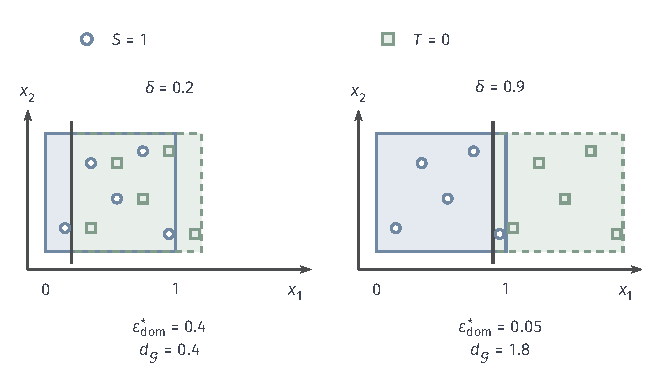
\includegraphics[width=113.404mm]{figures/06-foundations/02-learning-theory/tikz/learning-theory-domain-classifier/figure.pdf}
  \caption{域分类器的错误只对应输入散度项。源输入均匀分布于$[0,1]^2$，目标输入均匀分布于$[\delta,1+\delta]\times[0,1]$，其中$0\leq\delta\leq1$；圆点、方块的位置为教学构造，错误率由区域概率计算。$\mathcal H$含双向阈值与常值假设，域分类器类取$\mathcal G=\mathcal H\triangle\mathcal H$。其中$g=h_0\mathbin\oplus h_\delta$在左侧浅色带预测源域，$h_a(x)=\mathbb I\{x_1\geq a\}$；两域均等先验时，最小域错误为$(1-\delta)/2$，$d_{\mathcal G}=2\delta$。任务风险界还包含源风险及$\lambda=\inf_{h\in\mathcal H}(R_S(h)+R_T(h))$，不能只由域错误决定。}
  \label{fig:learning-domain-classifier}
\end{figure*}

\subsection{无目标数据的领域泛化}
\label{sec:domain-generalization}

训练和模型选择阶段都没有四月的任何数据时，就不能估计任意未知新域的密度比，正面结论只能依赖事先成立的关系，并且需要事先规定怎样评价新环境。这里比较两种不同的承诺。\term{逐目标域领域泛化}（target-wise domain generalization）要求同一学习程序对每个允许的目标域分别给出保证；\term{环境平均领域泛化}（environment-average domain generalization）把训练环境与新环境看成同一环境总体的随机抽样，评价新环境上的平均风险，后者允许某些环境风险较高。下面分别建立它们的来源、比较基准和有限样本结论。

\subsubsection{对允许目标域的统一保证}
\label{sec:dg-target-wise}

\paragraph{共同条件概率与非负超额损失}
设有若干个训练月份，它们按固定比例混合成训练分布$\overline{\mathcal P}$。对二分类零一损失，先考虑一个受控情形：训练混合与每个允许的目标域共享同一个条件正类概率$\eta(x)$，且Bayes分类器$h^\star(x)=\mathbb I\{\eta(x)\geq1/2\}$属于有限候选空间$\mathcal H$。两种邮件例子中的两个常值候选不满足后一条件，加入$h_{01}$以后才满足。

在固定输入$x$上，预测0、1的条件错误率分别为$\eta(x)$与$1-\eta(x)$；与Bayes决策不同所多付出的代价就是$|2\eta(x)-1|$。于是对任意域$D$，
\begin{equation}
 R_D(h)-R_D(h^\star)
 =\mathbb E_{\mathcal P_D^X}
   \bigl[|2\eta(x)-1|\,\mathbb I\{h(x)\neq h^\star(x)\}\bigr].
 \label{eq:dg-conditional-excess}
\end{equation}
被积函数非负，且只依赖共同的$\eta$与候选本身，与域无关；训练混合上的小超额风险不会由不同输入处的正负项相互抵消。为了防止未覆盖的输入再次出现，再要求每个允许目标都满足$\mathcal P_T^X\leq\kappa\overline{\mathcal P}^X$，即每个可测集合$B$都有$\mathcal P_T^X(B)\leq\kappa\overline{\mathcal P}^X(B)$。对非负被积函数，这个不等式逐集合成立便逐函数成立，于是
\[
 R_T(h)-R_T(h^\star)\leq\kappa\bigl[R_{\overline{\mathcal P}}(h)-R_{\overline{\mathcal P}}(h^\star)\bigr].
\]
又因为$h^\star$在每个域中都是全体可测决策中的最优者，并且属于$\mathcal H$，所以$R_T(h^\star)=R_{T,\mathcal H}^{\star}$，$R_{\overline{\mathcal P}}(h^\star)$也是训练混合上的类内最优值。

\begin{theorem}[共同Bayes候选下的逐目标域保证]
\label{thm:dg-target-wise}
在上述共享$\eta$、$h^\star\in\mathcal H$（$|\mathcal H|<\infty$）与统一覆盖常数$\kappa$的条件下，从训练混合$\overline{\mathcal P}$独立抽取$n$个样本，输出经验风险最小者$\widehat h$。则以概率至少$1-\delta$，对\emph{全部}允许目标域同时有
\[
 R_T(\widehat h)-R_{T,\mathcal H}^{\star}
 \leq\kappa\sqrt{\frac{2\log(2|\mathcal H|/\delta)}{n}} .
\]
\end{theorem}
\begin{proof}
训练样本来自$\overline{\mathcal P}$的独立同分布抽样，有限候选的Hoeffding估计与定理~\ref{thm:approximate-erm-risk}给出：以概率至少$1-\delta$，$R_{\overline{\mathcal P}}(\widehat h)-R_{\overline{\mathcal P}}(h^\star)\leq\sqrt{2\log(2|\mathcal H|/\delta)/n}$。在这个事件上，把上一段的覆盖不等式用于$h=\widehat h$，再代入$R_T(h^\star)=R_{T,\mathcal H}^{\star}$即得结论。成功事件只涉及训练样本，与目标域无关，所以同一个事件对全部允许目标同时成立。
\end{proof}

这一过程没有估计目标密度比：先在训练混合上学到接近共同Bayes候选的模型，再用统一覆盖常数把超额风险传到每个目标。由于成功事件只约束训练混合，结论比“逐个固定目标、各自高概率成立”更强。
\paragraph{各条件的作用与范围}
三个条件各自承担一步。共享$\eta$使式~\eqref{eq:dg-conditional-excess}中的权重$|2\eta-1|$在训练混合与目标域相同；$h^\star\in\mathcal H$使比较基准在每个域都是同一个候选；覆盖常数把输入比例的差别限制在因子$\kappa$之内。仅有相同的Bayes决策不足以完成这一步风险转换。设训练混合中$b$处$\eta(b)=1/2+\epsilon$，某个目标中$\eta(b)=1$，两域在$b$上的Bayes决策都是1。把$b$判为0的候选在训练混合上每单位概率只多付$2\epsilon$，在目标上却多付1；若允许族中$\epsilon$可以任意小，训练超额风险再小也不能控制目标超额风险，任何有限的转换常数都不存在。

共同Bayes候选的条件也强于“受限类中各域恰好有一个共同最优者”。若共同最优者不是Bayes决策，式~\eqref{eq:dg-conditional-excess}中的被积函数可以在不同输入处取不同符号，训练混合上的抵消在目标上未必发生。覆盖条件同样必须在所允许的目标族上一致：只对每个目标分别声称“存在某个有限常数”，常数可以随目标增大，就给不出统一的样本门槛。无目标数据时可以依靠的，正是这些事先成立的统一关系；它们不能从训练月份上观察到的经验不变性直接推出。

统计协议也要与证明一致。上面的结论要求从训练混合独立抽样。若改为每个训练月份固定取样数，各样本独立但不同分布，需要按相应的分层或独立非同分布观测重建偏差控制，再说明经验风险估计的是哪一种加权混合；不能直接套用混合分布的独立同分布样本界。

\subsubsection{随机新环境的平均保证}
\label{sec:dg-environment-average}

\paragraph{两层抽样与两项误差}
环境平均保证改变了评价对象：不再要求对任意指定的新月份都成功，而是把月份本身看成随机环境，评价一个共同模型在新抽月份上的平均风险。设先从环境总体$\mathcal Q$独立抽取$K$个分布$\mathcal P_1,\ldots,\mathcal P_K$，再从每个分布独立抽取$n$个观测，给定环境后不同块条件独立。模型在这些环境的经验平均上学习，评价
$R_{\mathcal Q}(h)=\mathbb E_{\mathcal P\sim\mathcal Q}R_{\mathcal P}(h)$。图~\ref{fig:learning-environment-sampling}区分环境数与域内样本数，它们对应两层随机性。

\begin{figure*}[!htb]
  \centering
  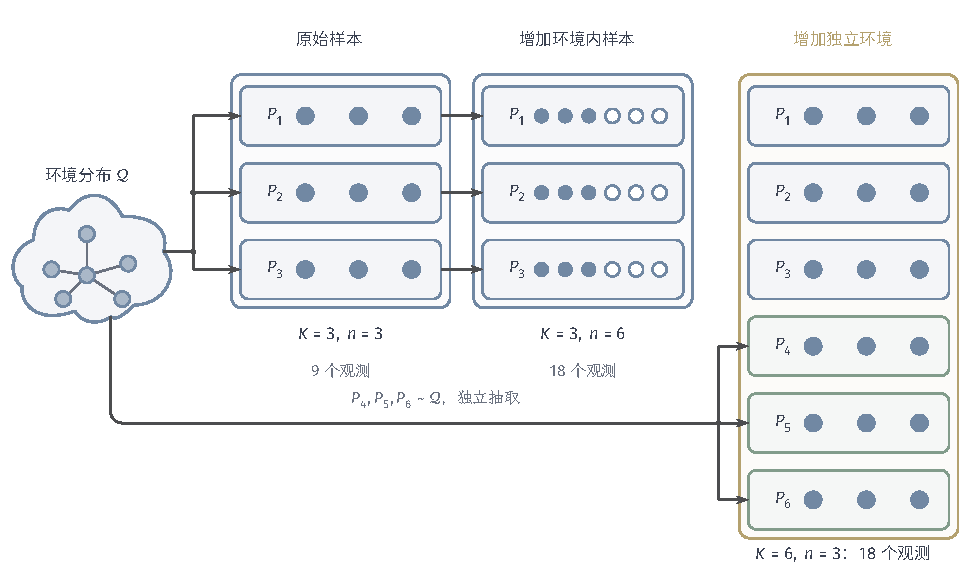
\includegraphics[width=164.600mm]{figures/06-foundations/02-learning-theory/tikz/learning-theory-environment-sampling/figure.pdf}
  \caption{环境数量$K$与环境内样本数$n$对应不同的抽样层。每行边界代表一个环境，圆点代表其中的观测。左侧从同一环境分布$\mathcal Q$独立抽取3个环境，各取3个观测；中间的空心点表示在原有3个环境中继续抽取的观测，每个环境增至6个；右侧从$\mathcal Q$新抽取3个独立环境，每个环境仍取3个观测。中、右都有18个观测，只有右侧增加了独立环境数量。图中数量为教学构造，不对应实测数据。}
 \label{fig:learning-environment-sampling}
\end{figure*}

记第$e$个环境的第$j$个观测为$z_{e,j}$，经验风险为
\[
 \widehat R(h)=\frac1{Kn}\sum_{e=1}^K\sum_{j=1}^n\ell(h,z_{e,j}).
\]
为区分两层抽样，引入已抽到环境的真实平均风险
\[
 R_K(h)=\frac1K\sum_{e=1}^K R_{\mathcal P_e}(h).
\]即使把每个环境的样本增加到无限多，经验风险也只是趋近这个随机的$R_K$，不一定等于环境总体风险。作分解
\[
 R_{\mathcal Q}(h)-\widehat R(h)
 =[R_{\mathcal Q}(h)-R_K(h)]+[R_K(h)-\widehat R(h)] ,
\]
两个差各自有对应的独立抽样单位。对包含$N$个候选、损失在$[0,1]$中的空间，第一项是$K$个独立环境风险的平均偏差，Hoeffding不等式和候选求和以失败概率至多$\delta/2$将其统一控制为$\sqrt{\log(4N/\delta)/(2K)}$。第二项先固定已抽到的环境，此时$Kn$个损失相互独立，平均期望正是$R_K(h)$；同样的方法给出$\sqrt{\log(4N/\delta)/(2Kn)}$，条件失败概率至多$\delta/2$，对环境抽样取平均后这个上界仍然成立。因此以概率至少$1-\delta$，
\begin{equation}
 \sup_h|R_{\mathcal Q}(h)-\widehat R(h)|
 \leq\sqrt{\frac{\log(4N/\delta)}{2K}}
     +\sqrt{\frac{\log(4N/\delta)}{2Kn}}.
 \label{eq:dg-two-level-uniform}
\end{equation}
给定环境后各损失未必同分布，但有界独立变量的Hoeffding分析仍然适用；不固定环境就把$Kn$个观测当成独立同分布抽样则不成立，因为同一块共享了随机环境。若算法近似最小化$\widehat R$、优化误差至多$\rho$，由定理~\ref{thm:approximate-erm-risk}，环境平均超额风险不超过右侧的两倍加$\rho$。比较基准是$\inf_hR_{\mathcal Q}(h)$，始终只选同一个候选，不能换成每个环境各选模型后的平均最优风险。

\paragraph{域内样本不能替代独立环境}
两种邮件的例子可以具体说明第一项的作用。令环境A只产生$a$邮件、环境B只产生$b$邮件，诈骗概率仍分别为0.1、0.9。环境总体以0.75的概率抽到A、0.25的概率抽到B，则两个常值候选的环境平均风险分别为$R_{\mathcal Q}(g_0)=0.75\times0.1+0.25\times0.9=0.3$与$R_{\mathcal Q}(g_1)=0.7$。若只抽一个训练环境，抽到B的概率为0.25；B内的独立样本增多时，经验风险最小者以趋于1的概率是$g_1$，其环境平均超额风险为0.4。增加域内样本把B的风险估计得越来越准，却改变不了“只见过B”这件事；只有增加独立环境才能减小这种机会。

在这个构造中，固定$g_0$的经验风险方差还可以精确分成$0.12/K+0.09/(Kn)$：前一项来自环境真实风险在0.1与0.9之间的变化，$0.75\times0.25\times0.8^2=0.12$；后一项来自给定环境后的标签抽样，$0.75\times0.09+0.25\times0.09=0.09$。它与式~\eqref{eq:dg-two-level-uniform}分离两种误差的做法一致，但不是该一般上界的等号情形。增大$n$只能消去第二项。

\paragraph{两种承诺的区别}
随机环境平均保证不是对任意指定目标域的保证。上面的例子中，即使学到了环境平均最优的$g_0$，它在环境B上的风险仍为0.9；环境平均只承诺“随机抽一个新月份时平均表现好”。分层观测也不能直接视为混合分布的独立同分布样本。评价协议改变以后，第~\ref{sec:dg-target-wise}节对每个允许目标同时成立的量词不能沿用；反过来，那里的共同Bayes候选与统一覆盖条件，这里也不需要。
\section{任务变化下的知识迁移}
\label{sec:task-transfer-learnability}

现在保持邮件及其诈骗标签的生成分布不变，只改变两类错误的代价。原来一次漏判和一次误拦受到相同惩罚，新的要求更重视减少误拦。若仍能访问全部带标签邮件，而且新代价已知，可以按新损失重新学习。迁移增加的问题是：旧任务只留下一个模型或一份摘要时，它是否足以支持新决策；若还需要新样本，又需要多少？本节先分清两种障碍：旧知识丢掉了所需信息，以及旧表示限制了能表达的决策（第~\ref{sec:task-information-needs}节）；再分别讨论不需要目标标签的直接转换（第~\ref{sec:task-risk-transfer}节）与利用目标标签的再次学习（第~\ref{sec:task-two-stage}节）；最后在同一基准下判断复用是否有收益（第~\ref{sec:task-transfer-benefit}节）。

\subsection{知识复用与目标任务的信息需求}
\label{sec:task-information-needs}

沿用邮件例子，一条完整观测$z=(x,y)$包含输入特征与诈骗标签。固定完整观测空间$Z$及其未知分布$\mathcal P$，让源任务与目标任务在共同候选空间$\mathcal H$上分别使用损失$\ell_S(h,z),\ell_T(h,z)\in[0,1]$，相应的总体风险为
\[
 R_S(h)=\mathbb E_{\mathcal P}\ell_S(h,z),\qquad
 R_T(h)=\mathbb E_{\mathcal P}\ell_T(h,z).
\]
本节下标$S,T$区分任务，两个期望中的分布始终相同；上一节用它们区分源域和目标域。若两个任务的输出形式不同，可以把$h$理解为包含所需输出的共同决策对象，再由损失读取相应部分；把两种输出放进同一个记号只统一了风险的写法，没有证明任务之间可以迁移。

源阶段接收$S_S\sim\mathcal P^{n_S}$，输出知识$K=A_S(S_S)$。$K$可以是类别预测器、概率预测器、把原始输入变为中间特征的映射$\phi_K$，也可以包含允许保留的统计摘要。目标算法接收$K$以及目标阶段的反馈$S_T$，输出$A_T(K,S_T)$。源样本已经进入$K$，但目标阶段不因此拥有这些样本的全部内容。复用最常见的形式是复用\term{表示}（representation）：$\phi_K$把邮件文本变成一组数值特征，目标阶段只在这些特征之上训练一个较简单的映射$g$，称为\term{预测头}（prediction head），目标候选是组合$g\circ\phi_K$。一般地，固定$K$以后只允许非空候选子集$\mathcal H_K\subseteq\mathcal H$，它由表示与允许的预测头共同确定。下面分别检查两件事：没有新标签时，$K$能否确定正确的目标决策；有标签时，$\mathcal H_K$能否表达所需决策。

\subsubsection{源任务最优结果的信息局限}
\label{sec:task-hard-label-limit}

先只考察一个输入，标签$y\in\{0,1\}$的正类概率记为$p$。允许两种未知的分布，分别取$p=0.6$与$p=0.9$。源任务使用零一损失，输出1的风险为$1-p$，输出0的风险为$p$，两种分布下唯一的源最优类别都是1。假设源阶段只保存这个类别，不保存风险值、概率估计或原始标签。

现在把“标签0判为1”（误拦）的代价设为0.8，把“标签1判为0”（漏判）的代价设为0.2，正确预测代价为0。预测1与预测0的目标风险分别为
\[
 R_T(1)=0.8(1-p),\qquad R_T(0)=0.2p ,
\]
二者之差为$R_T(1)-R_T(0)=0.8-p$，所以$p<0.8$时应输出0，$p>0.8$时应输出1。原来的阈值0.5已不足以支持新决策。数值可以直接复算：$p=0.6$时两个目标风险依次为0.32和0.12，错选1会多付0.2；$p=0.9$时依次为0.08和0.18，错选0会多付0.1。图~\ref{fig:lt9-hard-label-threshold}把两点放到同一条数轴上：它们都在0.5的右侧，所以存成同一个“类别1”；却分居0.8的两侧，要求相反的目标决策。源任务已经达到总体最优，信息缺口仍然存在，丢失的是概率上的区别，而不是源任务训练得不够充分。

\begin{figure}[htbp]
 \centering
 % 第9章：硬类别丢失概率信息。单个输入，正类概率 p 取 0.6 或 0.9。
% 源任务零一损失：p>0.5 时最优类别为 1（两种情形都存为“类别 1”）。
% 目标代价：标签0判1代价 0.8，标签1判0代价 0.2；R_T(1)=0.8(1-p)，R_T(0)=0.2p，阈值 0.8。
% p=0.6：R_T(1)=0.32, R_T(0)=0.12，应判 0；p=0.9：R_T(1)=0.08, R_T(0)=0.18，应判 1。
\begin{tikzpicture}[figure picture,x=1mm,y=1mm]
\def\L{75}
% 源任务决策带
\fill[FigureBlueFill] (0,21) rectangle (0.5*\L,25);
\fill[FigureRedFill] (0.5*\L,21) rectangle (\L,25);
\node[figure note,anchor=east] at (-2,23) {源任务};
\node[font=\figurefont\footnotesize] at (0.25*\L,23) {判 0};
\node[font=\figurefont\footnotesize] at (0.75*\L,23) {判 1};
% 目标任务决策带
\fill[FigureBlueFill] (0,3) rectangle (0.8*\L,7);
\fill[FigureRedFill] (0.8*\L,3) rectangle (\L,7);
\node[figure note,anchor=east] at (-2,5) {目标任务};
\node[font=\figurefont\footnotesize] at (0.4*\L,5) {判 0};
\node[font=\figurefont\footnotesize] at (0.9*\L,5) {判 1};
% 数轴
\draw[FigureStroke,line width=.75pt] (0,13) -- (\L,13);
\foreach \v in {0,0.5,0.8,1}{\draw[FigureStroke,line width=.6pt] (\v*\L,12) -- (\v*\L,14);}
\node[figure note,anchor=east] at (-2,13) {$p$};
\node[font=\figurefont\footnotesize,anchor=north] at (0,12) {0};
\node[font=\figurefont\footnotesize,anchor=north] at (\L,12) {1};
\draw[FigureStroke,line width=.6pt,dash pattern=on 2pt off 1.5pt] (0.5*\L,12) -- (0.5*\L,26);
\draw[FigureStroke,line width=.6pt,dash pattern=on 2pt off 1.5pt] (0.8*\L,1) -- (0.8*\L,14);
\node[figure note] at (0.5*\L,28) {源阈值 0.5};
\node[figure note] at (0.8*\L,-1.5) {新阈值 0.8};
% 两个可能的概率
\foreach \v/\t in {0.6/{$p=0.6$},0.9/{$p=0.9$}}{%
  \fill[FigureInk] (\v*\L,13) circle (1mm);
  \node[font=\figurefont\footnotesize] at (\v*\L,16.8) {\t};}
% 保存的硬类别
\node[figure note,align=left,anchor=west] at (\L+3,23) {两点都存为\\“类别 1”};
\node[figure note,align=left,anchor=west] at (\L+3,5) {两点要求\\相反决策};
\end{tikzpicture}

 \caption{硬类别丢失新阈值所需的概率信息。数轴为正类概率$p$；上带是源任务零一损失的决策区域（阈值0.5），下带是误拦代价0.8、漏判代价0.2时的目标决策区域（阈值0.8）。$p=0.6$与$p=0.9$在源任务中都存为“类别1”，在目标任务中应分别判0与判1。}
 \label{fig:lt9-hard-label-threshold}
\end{figure}

把这个缺口写成学习协议下的失败。固定“只读旧类别、没有新标签”的协议：目标算法收到的唯一信息是“类别1”，它在两种分布下相同。若算法以概率$q$输出1，那么在$p=0.6$的分布下，它以概率$q$产生0.2的目标超额风险；在$p=0.9$的分布下，它以概率$1-q$产生0.1的超额风险。要求精度$\varepsilon<0.1$时，两个失败概率$q$与$1-q$至少有一个不小于$1/2$，统一的失败概率$\delta<1/2$无法达到。增加源样本却仍只保留最优类别，不会改变这份知识。保存概率或提供目标标签都改变了可用信息，后面分别分析这两条正面路径。

这里没有把任务改变解释为分布改变。在每一种可能的世界中，$p$在两个任务间始终固定；比较两个世界，是为了检查同一算法能否对未知分布统一成功。反例说明“源最优类别”这种知识载体不足，并不是说任何源知识都不能迁移。

\subsubsection{固定表示与目标近似差}
\label{sec:task-representation-gap}

前一个反例说的是没有新标签时的信息不足。即使目标标签无限多，固定表示也可能限制最终能实现的决策。把两个可能的概率放进同一个分布：输入$a,b$各以概率$1/2$出现，条件正类概率分别为0.6、0.9；源任务仍使用零一损失。源最优分类器在两点都输出1，所以一个把两点映射到同一特征的常值表示$\phi_K(a)=\phi_K(b)$，配上常值预测头，已经足以实现源最优分类。

目标代价仍取0.8与0.2。若大空间$\mathcal H$包含两点上的全部四个二分类函数，目标最优者在$a$输出0、在$b$输出1。表示合并两点以后，任何预测头只能给它们相同的类别。图~\ref{fig:lt9-representation-merge}列出逐点的条件风险和总风险：原空间最优风险为$\tfrac12\times0.12+\tfrac12\times0.08=0.10$，合并后两个常值决策的风险为$\tfrac12(0.12+0.18)=0.15$与$\tfrac12(0.32+0.08)=0.20$。即使目标算法完全知道这个分布，受限空间的最小风险仍为0.15，比原空间高0.05。这部分差距来自表示合并输入，而不是目标样本不足。

\begin{figure}[htbp]
 \centering
 % 第9章：固定表示合并输入造成近似差。输入 a,b 各以 1/2 出现，eta(a)=0.6, eta(b)=0.9。
% 目标代价 0.8（0判1）、0.2（1判0）。逐点条件风险：a 上判1为0.32、判0为0.12；b 上判1为0.08、判0为0.18。
% 原空间最优 (a->0,b->1)：(0.12+0.08)/2=0.10；常值0：(0.12+0.18)/2=0.15；常值1：(0.32+0.08)/2=0.20。
% 近似差 a_T(K)=0.15-0.10=0.05。
\begingroup
\definecolor{FigureGreenFill}{HTML}{E8EEE9}
\begin{tikzpicture}[figure picture,x=1mm,y=1mm]
\node[draw=FigureBlue,fill=FigureBlueFill,circle,minimum size=8mm,inner sep=0pt] (a) at (4,26) {$a$};
\node[draw=FigureBlue,fill=FigureBlueFill,circle,minimum size=8mm,inner sep=0pt] (b) at (4,8) {$b$};
\node[figure note,anchor=north] at (4,21.5) {$\eta=0.6$};
\node[figure note,anchor=north] at (4,3.5) {$\eta=0.9$};
\node[draw=FigureYellow,fill=FigureYellowFill,rounded corners=1.5mm,minimum width=12mm,minimum height=8mm] (u) at (30,17) {$u$};
\draw[figure flow] (a) -- (u);
\draw[figure flow] (b) -- (u);
\node[font=\figurefont\footnotesize] at (17,17) {$\phi_K$};
\node[draw=FigureRed,fill=FigureRedFill,rounded corners=1.5mm,minimum width=12mm,minimum height=8mm] (o) at (48,17) {0 或 1};
\draw[figure flow] (u) -- node[figure edge label,above] {$g$} (o);
\node[figure note,align=center] at (30,6) {两点被\\合成同一特征};
% 风险表
\begin{scope}[shift={(60,0)}]
\foreach \x/\w/\t in {0/18/{决策},18/10/{$a$上},28/10/{$b$上},38/12/{$R_T$}}{%
  \node[draw=FigureGrid,minimum width=\w mm,minimum height=6.2mm,inner sep=0pt,anchor=north west,font=\figurefont\footnotesize] at (\x,32) {\t};}
\foreach \y/\d/\ra/\rb/\r/\f in {25.8/{$a\!\to\!0,\ b\!\to\!1$}/0.12/0.08/0.10/FigureGreenFill,
                                 19.6/{恒判 0}/0.12/0.18/0.15/FigureYellowFill,
                                 13.4/{恒判 1}/0.32/0.08/0.20/white}{%
  \node[draw=FigureGrid,minimum width=18mm,minimum height=6.2mm,inner sep=0pt,anchor=north west,font=\figurefont\footnotesize] at (0,\y) {\d};
  \node[draw=FigureGrid,minimum width=10mm,minimum height=6.2mm,inner sep=0pt,anchor=north west,font=\figurefont\footnotesize] at (18,\y) {\ra};
  \node[draw=FigureGrid,minimum width=10mm,minimum height=6.2mm,inner sep=0pt,anchor=north west,font=\figurefont\footnotesize] at (28,\y) {\rb};
  \node[draw=FigureGrid,fill=\f,minimum width=12mm,minimum height=6.2mm,inner sep=0pt,anchor=north west,font=\figurefont\footnotesize] at (38,\y) {\r};}
\node[figure note,anchor=north west,align=left] at (0,5.5) {绿：原空间最优；黄：合并后最优；\\两者之差 $a_T(K)=0.05$};
\end{scope}
\end{tikzpicture}
\endgroup

 \caption{固定表示合并输入造成的近似差。输入$a,b$各以概率$1/2$出现，$\eta(a)=0.6$、$\eta(b)=0.9$；表示$\phi_K$把两点映到同一特征$u$，预测头$g$只能对它们输出同一类别。右表为误拦代价0.8、漏判代价0.2时各决策的逐点条件风险与总目标风险$R_T$；原空间最优为0.10，合并后最优为0.15，差$a_T(K)=0.05$。}
 \label{fig:lt9-representation-merge}
\end{figure}

为了在一般问题中保留这项代价，对非空的$\mathcal H_K\subseteq\mathcal H$定义
\begin{equation}
 a_T(K)=\inf_{h\in\mathcal H_K}R_T(h)
        -\inf_{h\in\mathcal H}R_T(h)\geq0 .
 \label{eq:task-transfer-bias}
\end{equation}
两个下确界都按目标风险选择最好候选，但前者只能使用保留下来的表示与允许的预测头；$a_T(K)$衡量这项限制使最佳可达风险增加了多少，两点例子中它正好是0.05。$a_T(K)=0$只要求受限空间能够任意逼近大空间的最优风险，不要求最小者存在。这个差同时取决于表示和预测头：即使保留原始输入，若只允许常值预测头，差距仍然存在；保留两点的区别并允许全部二分类预测头，才把它降为0。所以不能单凭表示维数或源准确率断言$a_T(K)$小。

后文统一用大空间基准$R_{T,\mathcal H}^{\star}=\inf_{h\in\mathcal H}R_T(h)$评价迁移。若只看相对于$\mathcal H_K$的类内超额风险，单元素空间总能取得零类内超额风险，即使这个唯一候选在目标任务上始终出错；大空间基准使表示限制造成的损失留在评价中。
\subsection{无需目标标签的风险转换}
\label{sec:task-risk-transfer}

现在固定一种协议：新损失已知，目标阶段只读取旧知识，不再收到任何标签。这时需要一条可以执行的决策转换，以及一条把源风险联系到目标风险的不等式。先给一般的充分条件，再用概率知识支持代价变化的例子说明这种关系怎样建立。

\subsubsection{候选转换与超额风险关系}

记源任务的类内基准为$R_{S,\mathcal H}^{\star}=\inf_{h\in\mathcal H}R_S(h)$。若已知可计算的候选转换$\Gamma:\mathcal H\to\mathcal H$和统一常数$c,b\geq0$，并能对每个$h\in\mathcal H$及允许的每个分布与任务对证明
\begin{equation}
 R_T(\Gamma(h))-R_{T,\mathcal H}^{\star}
 \leq c\bigl(R_S(h)-R_{S,\mathcal H}^{\star}\bigr)+b ,
 \label{eq:task-risk-transfer}
\end{equation}
那么源超额风险不超过$\varepsilon_S$的成功事件，直接包含于“目标超额风险不超过$c\varepsilon_S+b$”的事件。这种保证不需要目标标签，但要求转换规则已知、可以实施，而且不等式在允许族上一致成立；只对某一个分布对成立的关系，不能给出统一的样本门槛。

最简单的例子是正仿射变化。当$\ell_T(h,z)=c\,\ell_S(h,z)+d(z)$、$c>0$，且$d$与决策无关、期望有限时，$R_T(h)=cR_S(h)+\mathbb E d(z)$。对候选取下确界，同一个常数也出现在最优风险中，相减得$R_T(h)-R_{T,\mathcal H}^{\star}=c(R_S(h)-R_{S,\mathcal H}^{\star})$，转换取恒等映射，$b=0$。这时两种目标的最优排序完全相同，比较候选和基准都没有变化。前面的误判代价调整不属于这种情形：误拦与漏判的代价按不同比例改变，排序随之改变，不能沿用源最优类别。

把源学习保证代入式~\eqref{eq:task-risk-transfer}即得目标保证：若源程序以概率至少$1-\delta$达到源超额风险$\varepsilon_S$，所需样本数为$m_S(\varepsilon_S,\delta)$，则在同一事件上目标超额风险至多$c\varepsilon_S+b$。要达到目标精度$\varepsilon>b$，取$\varepsilon_S=(\varepsilon-b)/c$即可，源样本需求为$m_S((\varepsilon-b)/c,\delta)$，失败概率不变。$b$是这条转换能证明的精度下限；当$\varepsilon\leq b$时，这条路线给不出结论。若转换只有充分界，不能由残余$b$推出所有算法都无法学习。

\subsubsection{条件概率与代价敏感决策}
\label{sec:task-probability-transfer}

\paragraph{概率误差控制新阈值的代价}
对代价改变，更有用的源知识是条件概率。仍令$\eta(x)=\mathbb P(y=1\mid x)$，让源阶段输出$f(x)\in[0,1]$，并用平方损失$(f(x)-y)^2$训练。要得到新阈值决策的保证，先判断源平方风险能控制概率估计的哪一种误差。本小节把$f$与真实的$\eta$比较，把目标决策与全部可测决策中的Bayes最优者比较。

给定输入$x$，把预测误差写成$f(x)-y=[f(x)-\eta(x)]+[\eta(x)-y]$。平方后取条件期望，交叉项为$2[f(x)-\eta(x)]\,\mathbb E[\eta(x)-y\mid x]=0$。再对输入取期望，得到
\[
 \begin{aligned}
 R_S(f)&=\mathbb E[(f(x)-\eta(x))^2]+\mathbb E[(\eta(x)-y)^2],\\
 R_S(f)-R_S(\eta)&=\mathbb E[(f(x)-\eta(x))^2].
 \end{aligned}
\]
第二项是标签在给定输入后仍有的随机波动，不随$f$改变。所以源平方超额风险恰好是概率估计的均方误差，源阶段可以把这项信息交给新任务。

设目标任务把误拦的代价记为$c_0\in(0,1]$，把漏判的代价记为$c_1\in(0,1]$。给定$x$，决策1与决策0的条件风险分别为$c_0(1-\eta(x))$与$c_1\eta(x)$，比较二者得到阈值$\tau=c_0/(c_0+c_1)$；按真实概率决策时，$d_\eta(x)=\mathbb I\{\eta(x)\geq\tau\}$达到Bayes最优，等号处选1只是固定的平局规则。前面的例子中$c_0=0.8$、$c_1=0.2$，$\tau=0.8$。

目标阶段没有$\eta$，但可以用保留下来的$f$构造$d_f(x)=\mathbb I\{f(x)\geq\tau\}$。若$d_f=d_\eta$，这个输入上没有额外损失；若二者不同，选错决策增加的条件风险是$|c_0(1-\eta)-c_1\eta|=(c_0+c_1)|\eta(x)-\tau|$。发生这种分歧时，阈值必然位于$f(x)$与$\eta(x)$之间，所以$|\eta(x)-\tau|\leq|f(x)-\eta(x)|$：即使某个概率误差改变了类别，它造成的代价仍受这项概率误差控制。逐输入取期望，再用Cauchy--Schwarz不等式，
\begin{align*}
 R_T(d_f)-R_T(d_\eta)
 &= (c_0+c_1)\,\mathbb E\bigl[|\eta(x)-\tau|\,
       \mathbb I\{d_f(x)\neq d_\eta(x)\}\bigr] \\
 &\leq(c_0+c_1)\,\mathbb E|f(x)-\eta(x)| \\
 &\leq(c_0+c_1)\sqrt{R_S(f)-R_S(\eta)} .
\end{align*}
这条不等式把源平方风险、保留的概率和目标代价风险接成一条完整关系，它是式~\eqref{eq:task-risk-transfer}在“转换$=$移动阈值”时的平方根形式。新代价已知时，只需移动阈值，不必重新估计标签分布。回到图~\ref{fig:lt9-hard-label-threshold}：硬类别只报告$\eta$位于0.5的哪一侧，保存$f$则保留了判断$\eta$位于0.8哪一侧所需的信息。

\paragraph{源样本量与收敛速度}
上式的基准是$\eta$本身，而$f$只能来自某个源概率类。设源概率类$\mathcal F$包含$N_S$个$[0,1]$值函数，源算法在$n_S$个完整观测上近似最小化平方经验风险，优化误差至多$\rho_S$。记其相对于真实概率的近似差为$\alpha_{\mathcal F}=\inf_{f\in\mathcal F}R_S(f)-R_S(\eta)$。平方损失属于$[0,1]$，对全部源候选使用Hoeffding不等式，再由定理~\ref{thm:approximate-erm-risk}比较经验近似最小者与类内最小者，以概率至少$1-\delta_S$，
\[
 R_S(f)-R_S(\eta)
 \leq\alpha_{\mathcal F}
     +\sqrt{\frac{2\log(2N_S/\delta_S)}{n_S}}+\rho_S .
\]
代入平方根转换，同一事件上目标超额风险至多$(c_0+c_1)$乘以右侧的平方根。若目标比较空间$\mathcal H$包含$d_\eta$，Bayes风险就是$R_{T,\mathcal H}^{\star}$，这个界也是相对于大空间基准的超额风险；否则它控制的是相对于Bayes风险的差，类内基准只会更低。这条路径只使用源标签和已知的目标代价。

若$\alpha_{\mathcal F}$与$\rho_S$为零，有限源类与置信水平固定，目标超额风险的充分界为$(c_0+c_1)\,[2\log(2N_S/\delta_S)/n_S]^{1/4}$，按源样本量的负四分之一次幂下降。要使它不超过$\varepsilon$，反解得
\[
 n_S\geq\frac{2(c_0+c_1)^4\log(2N_S/\delta_S)}{\varepsilon^4}
\]
就足够。这个速率来自通用估计界再经平方根转换，不是这类问题最优样本复杂度的刻画；更精细的概率学习分析，或对阈值附近标签规律的附加条件，都可能支持更快的结论。另一方面，若$\alpha_{\mathcal F}$或$\rho_S$固定为正，例如$\mathcal F$根本不能逼近$\eta$，目标界中就留下$(c_0+c_1)\sqrt{\alpha_{\mathcal F}+\rho_S}$的固定正残余，增加源样本不能从当前上界中消除它；平方风险相对于$\mathcal F$自身已经最优，并不足以把它降为零。
\subsection{利用目标样本的两阶段学习}
\label{sec:task-two-stage}

当目标阶段能取得计算新损失所需的标签时，可以在旧知识确定的候选空间$\mathcal H_K$中再次学习，例如在固定表示上重新训练预测头。先条件于知识分析目标学习，再把源阶段随机知识的质量纳入总保证；两阶段使用同一个大空间基准。

\subsubsection{固定知识后的目标学习保证}

为把源知识的误差与目标样本的估计误差分开，令目标样本$S_T=(z_1,\ldots,z_n)\sim\mathcal P^n$与$S_S$独立，并提供计算$\ell_T$所需的完整反馈。条件于$K$以后，$\mathcal H_K$固定，目标样本仍独立同分布。对任意输出$\widehat h\in\mathcal H_K$先作恒等分解：
\[
 R_T(\widehat h)-R_{T,\mathcal H}^{\star}
 =a_T(K)+\Bigl[R_T(\widehat h)-\inf_{h\in\mathcal H_K}R_T(h)\Bigr].
\]
第一项问保留知识以后还容许多好的目标候选，第二项问目标算法能否从这批候选中学到接近最好的一个。目标样本可以减小后一项，却不能改变已经固定的候选集合。设每个可能的$K$都确定有限非空空间$\mathcal H_K$，且$|\mathcal H_K|\leq N_0$；对每个候选计算目标经验风险$\widehat R_T(h)=n^{-1}\sum_{i=1}^n\ell_T(h,z_i)$。

\begin{theorem}[复用知识后的目标风险保证]
\label{thm:task-transfer-finite}
设$K$与目标样本$S_T\sim\mathcal P^n$独立，$\mathcal H_K\subseteq\mathcal H$满足上述大小限制，目标损失可测且属于$[0,1]$。若输出$\widehat h\in\mathcal H_K$满足$\widehat R_T(\widehat h)\leq\min_{h\in\mathcal H_K}\widehat R_T(h)+\rho$，则以概率至少$1-\delta$，
\begin{equation}
 R_T(\widehat h)-R_{T,\mathcal H}^{\star}
 \leq a_T(K)+\sqrt{\frac{2\log(2N_0/\delta)}{n}}+\rho .
 \label{eq:task-transfer-finite}
\end{equation}
\end{theorem}
\begin{proof}
先条件于$K$，此时$\mathcal H_K$固定。对每个候选使用Hoeffding不等式，再对至多$N_0$个候选的失败事件求和，得到条件概率至少$1-\delta$的共同事件：
\[
 \sup_{h\in\mathcal H_K}|\widehat R_T(h)-R_T(h)|
 \leq a_n=\sqrt{\frac{\log(2N_0/\delta)}{2n}} .
\]
有限非空集合中存在目标风险最小者$h_K^\star$。在这个事件上，按定理~\ref{thm:approximate-erm-risk}的三步比较，
\[
 R_T(\widehat h)\leq\widehat R_T(\widehat h)+a_n
 \leq\widehat R_T(h_K^\star)+\rho+a_n
 \leq R_T(h_K^\star)+\rho+2a_n .
\]
减去大空间最优风险后，$R_T(h_K^\star)-R_{T,\mathcal H}^{\star}$正是$a_T(K)$。对每个$K$，条件失败概率都至多$\delta$，再对源知识取平均，联合失败概率仍至多$\delta$。
\end{proof}

独立性保证源阶段选了哪一组候选，不会改变目标样本在给定$K$后的分布。若已知$a_T(K)\leq b$且$b+\rho<\varepsilon$，那么
\[
 n\geq\frac{2\log(2N_0/\delta)}{(\varepsilon-b-\rho)^2}
\]
是目标精度$\varepsilon$的充分样本量。近似差与优化误差占用了可用于抽样误差的精度预算；二者之和达到$\varepsilon$时，这条界不能靠增加$n$给出所需保证。特别地，$a_T(K)=\rho=0$时，样本需求恢复为$2\log(2N_0/\delta)/\varepsilon^2$。在两点例子中，$a_T(K)=0.05$，所以要求$\varepsilon\leq0.05$时，无论目标样本多少都不可能，这是候选限制造成的不可达精度，与统计上界没有下降到所需数值不同。

计算方面，候选损失可计算且可比较时，枚举$N_0$个候选、各算$n$个损失即可取$\rho=0$，损失评估次数为$nN_0$。这是可执行的充分构造，不是高效求解任意表示模型的结论。预测头为无限集合时，可以用第~\ref{sec:rademacher-complexity}节的复杂度代替$\log N_0$，这时控制的是\emph{固定知识后的目标损失类}$\{\ell_T(g\circ\phi_K,\cdot)\}$，复杂度随$K$变化，条件于$K$计算。预测头较小可能降低估计代价，但不保证近似差小，也不保证经验目标容易优化；优化保证需另行证明。

\subsubsection{源知识质量与两阶段总体保证}

$K$由随机源样本得到，所以$a_T(K)$也是随机的。若源阶段的分析证明$\mathbb P\{a_T(K)\leq b_S(n_S,\delta_S)\}\geq1-\delta_S$，目标阶段再对每个固定的$K$以条件失败概率至多$\delta_T$控制类内学习误差，两项保证就可以在失败概率至多$\delta_S+\delta_T$的事件外合并。这里$b_S$必须由源学习与任务联系共同推出，源经验风险小不能直接替代这个结论。

第~\ref{sec:task-probability-transfer}节提供了一个现成的$b_S$。若$\mathcal H_K$至少包含按新代价构造的$d_f$，则
\[
 a_T(K)\leq R_T(d_f)-R_{T,\mathcal H}^{\star}\leq R_T(d_f)-R_T(d_\eta)
 \leq(c_0+c_1)\sqrt{R_S(f)-R_S(\eta)} ,
\]
第一个不等式用$\mathcal H_K\ni d_f$，第二个用大空间最优风险不低于Bayes风险。再代入那里的源概率保证，就得到随源样本量下降的$b_S$，无需另外假设一个与源学习无关的表示质量。例如，若同一源程序能用$n_S$个样本以概率至少$1-\delta/2$保证$a_T(K)\leq\varepsilon/3$，所有$\mathcal H_K$的大小至多$N_0$，再令目标优化误差不超过$\varepsilon/3$，则由定理~\ref{thm:task-transfer-finite}，$n_T\geq18\log(4N_0/\delta)/\varepsilon^2$足以把目标抽样项控制在$\varepsilon/3$以内。失败事件相加不超过$\delta$，三项风险预算相加不超过$\varepsilon$。

目标样本独立于源阶段是这里的分析条件，不是任务改变所必需的代价：若旧的原始数据仍完整保留、且新损失能在上面计算，也可以按相应协议直接重新学习。对允许的任务族给出统一结论时，需要固定允许的分布与任务对集合$\mathfrak T$，要求存在同一源程序、同一目标程序和有限门槛$m_S,m_T$，使对每个$\varepsilon,\delta$、每个$(\mathcal P,\ell_S,\ell_T)\in\mathfrak T$及足够大的$n_S,n_T$，都有
\[
 \mathbb P\{R_T(A_T(K,S_T))-R_{T,\mathcal H}^{\star}\leq\varepsilon\}\geq1-\delta .
\]
门槛可以依赖任务族的统一参数，但不能依赖未知的具体分布；对每个已经实现的$K$分别控制目标学习误差，还没有证明源程序能统一产生足够小的$a_T(K)$。另一处容易出错的地方是数据复用：若用同一批目标数据反复挑选源模型或修改表示，再把最终的候选集合当作抽样前固定的集合估计风险，就漏算了这些选择的代价。此时需要对全部可能的选择作统一控制，或用新的独立数据进行评价。

\subsection{迁移收益与负迁移}
\label{sec:task-transfer-benefit}

“目标任务能学会”与“复用知识有收益”是两个问题。在相同目标损失、相同风险基准与相同新增样本预算下比较直接学习与复用：直接学习在大小为$N$的$\mathcal H$中选择，复用在大小至多$N_0<N$的$\mathcal H_K$中选择。有限候选界把$\log(2N/\delta)$换成$\log(2N_0/\delta)$，这解释了有用的知识怎样减少目标阶段需要区分的候选；但近似差$a_T(K)$同时占用精度预算。取$N=2^{20}$、$N_0=2^{10}$、$\delta=0.05$、$\varepsilon=0.1$并令$\rho=0$：直接学习的充分样本量约为$2\log(2^{21}/0.05)/0.01\approx3.5\times10^3$，复用且$a_T(K)=0$时约为$2\log(2^{11}/0.05)/0.01\approx2.1\times10^3$；若$a_T(K)=0.05$，则变为$2\log(2^{11}/0.05)/0.05^2\approx8.5\times10^3$，反而更多。估计收益与近似代价必须一起评价。两个充分上界的大小也不能证明最优样本复杂度的严格排序，它们只说明各自路线能保证什么。

成本还要按阶段分列。源阶段已经消耗的$n_S$个样本和训练计算不能算作不存在。若只完成一个新任务，源训练的额外成本可能超过目标阶段的节省；若同一知识服务多个目标任务，就要同时统计源总成本与各任务的新增成本，收益还取决于这些任务是否共享同一份可复用的结构。共享表示理论研究源任务的多样性何时足以支持这种复用，并在相应的任务联系下控制新任务的样本需求\scite{tripuraneni2020diversity}。要把任意新损失都纳入目标任务族，需要比只覆盖特定任务族更强的信息保留条件。

若复用源知识以后，目标风险反而高于不用这份知识直接学习，就称发生了\term{负迁移}（negative transfer）。上面的分解给出它的一种来源：$a_T(K)$过大，节省下来的估计误差抵不过表示限制带来的近似差。判断负迁移时，应在相同目标样本、评价分布和可比训练预算下比较实际目标风险，或比较明确定义的理论风险差；迁移路线的上界更松，并不等于已经发生负迁移，因为上界只是充分条件，不是实际风险。

最后对照三种复用方式。冻结表示时，预测空间固定为$\mathcal H_K$，目标数据只选预测头，前两小节的保证直接适用。部分更新表示时，预测空间扩大到以$K$为起点、允许改变的那部分参数所能达到的集合，它由目标数据决定，近似差可能缩小，统计控制须覆盖更大的候选集合，求解条件也随之改变。完全重新学习则回到大空间$\mathcal H$，旧知识至多提供初始化。三者改变的是预测空间、数据依赖与求解条件这三项中的哪几项，前两条保证据此判断是否适用；具体的训练算法留给相应的范式和模型章节。
\section{历史访问受限的持续学习}
\label{sec:continual-learnability}

继续按月份接收邮件，并要求模型仍能处理已经出现过的邮件类型。新数据能帮助调整当前决策，但旧邮件离开以后，算法不能再用它们检查每次调整是否损害了历史预测。本节先固定数据到达方式、状态更新与评价时点，定义要承担的历史风险（第~\ref{sec:continual-protocol}节）；再区分两种失败来源：没有一个预测器能同时完成要求，以及有限状态没有保留选出它所需的信息（第~\ref{sec:continual-conditions}节）；在条件允许时，对固定的有限候选分别构造支持历史平均目标与逐域目标的摘要和保证（第~\ref{sec:continual-fixed-candidates}节）；最后说明只做局部参数更新时，还需怎样控制长期遗忘（第~\ref{sec:continual-repeated-updates}节）。

\subsection{序列学习与历史风险}
\label{sec:continual-protocol}

本小节固定数据到达方式、状态更新与评价时点。历史责任由任务规定：若任务只要求当前月份的风险小，历史错误率上升并不违反承诺；若要求覆盖历史邮件，就要明确是平均覆盖还是逐月覆盖。不能仅凭“持续更新”就认定算法必须满足某种特定的保持要求。

\subsubsection{数据阶段、状态与预测协议}

固定输入空间$X$、标签空间$Y$、候选空间$\mathcal H$和损失$\ell(h,z)\in[0,1]$，其中$z=(x,y)$。第$t$阶段收到$S_t=(z_{t,1},\ldots,z_{t,n_t})$，其观测来自分布$\mathcal P_t$。任务固定是指输入输出的含义和损失不随阶段改变；$\mathcal P_t$仍可以改变输入比例、标签比例或条件标签概率，始终不变也是一种情形。每个阶段结束后，算法留下足以支持下一次更新和预测的全部信息，记为状态$M^{(t)}$：
\[
 M^{(t)}=U_t(M^{(t-1)},S_t),\qquad
 h^{(t)}=V_t(M^{(t)}).
\]
$U_t$接收旧状态与新样本并更新状态，$V_t$从状态中取出当前预测规则；带括号的上标表示阶段。模型参数、保留样本和历史统计量都包含在$M^{(t)}$中。样本离开以后，更新只能通过这个状态取得历史信息。

正面结论先固定一条不依赖训练样本的分布序列$\mathcal P_1,\ldots,\mathcal P_T$：阶段内样本独立同分布，不同阶段的样本相互独立。分布可以缓慢改变、突然改变或始终不变，只要求这种选择不依赖已经抽到的样本；若模型输出会反过来改变下一阶段的数据，需要在相应的条件信息下重新分析。本节约定预测时不提供环境身份，即同一个$h^{(t)}$承担全部历史分布上的预测；若提供身份并允许据此调用不同模型，候选空间和存储要求都会改变，那是另一个学习问题。

评价发生在第$t$阶段更新完成以后：$h^{(t)}$在各分布中新观测上的期望损失。评价样本不参与这次训练，总体风险通过分布定义，并不要求算法持有一套无限测试集。这与先预测、后收到标签的在线协议不同，后者还要计入反馈前已经发生的错误；本节的保证也不覆盖尚未观察到的第$t+1$阶段分布。资源方面，要事先约定允许的分布序列族、阶段上限$T$与记忆预算。有限维参数不自动意味着有限比特状态：一个实数向量若用无限精度编码全部过去，就不能当作有限记忆。模型描述、保留样本以及数据相关的摘要，都应按协议计入资源；固定候选的程序描述可以预先给定，但从数据中选中了哪个候选仍属于状态。

\subsubsection{当前风险、历史风险与遗忘}
\label{sec:continual-risks}

用一个没有抽样噪声的小例子比较几种评价。输入只有$a,b$：三月恒产生$(a,0)$，四月恒产生$(b,1)$。候选空间包含四个分类器$h_{00},h_{01},h_{10},h_{11}$，下标依次给出它们对$a,b$的预测，例如$h_{01}(a)=0$、$h_{01}(b)=1$。记$R_i(h)=\mathbb E_{\mathcal P_i}\ell(h,z)$为第$i$阶段总体上的风险，$R_i^\star=\inf_{h\in\mathcal H}R_i(h)$；这里$R_1^\star=R_2^\star=0$。\emph{当前风险}是$R_t(h^{(t)})$。为让每个已出现的阶段在评价中占相同权重，定义\emph{历史平均风险}
\begin{equation}
 \overline R_t(h)=\frac1t\sum_{i=1}^tR_i(h) ;
 \label{eq:continual-average-risk}
\end{equation}
若实际部署频率不同，可以事先规定其他权重，但随后使用的经验量也必须估计同一组权重下的风险。要求每个历史分布都接近各自最优时，评价\emph{最大逐域超额风险}
\[
 E_t(h)=\max_{i\leq t}[R_i(h)-R_i^\star].
\]
最后，比较同一历史环境上更新前后的风险，定义\term{遗忘}（forgetting）$F_{i,t}=R_i(h^{(t)})-R_i(h^{(i)})$，$i<t$；正值表示完成第$i$阶段学习以后，该阶段的风险有所增加，负值表示后来的更新改善了它。

图~\ref{fig:lt9-continual-four-classifiers}比较第二阶段结束时的四种结果。前三行都从$h^{(1)}=h_{00}$出发。冻结旧模型保持$h_{00}$，风险$(R_1,R_2)=(0,1)$：历史能力没有下降，当前却没有学会。只适应当前改用$h_{11}$，风险变为$(1,0)$：当前完全正确，三月的能力全部丢失，$F_{1,2}=1$。兼顾新旧选$h_{01}$，达到$(0,0)$。末行从三月起始终使用$h_{10}$，三月风险一直为1，遗忘却为0。所以遗忘要与绝对风险或超额风险一起读：变化小不能说明原先已经学好。保持参数或只优化当前数据，都不足以确定整个过程是否成功；保持与适应须同时检查对应的风险。

\begin{figure*}[htbp]
 \centering
 % 第9章：持续学习中四个分类器的风险表。第1阶段恒产生 (a,0)，第2阶段恒产生 (b,1)，零一损失。
% h_{uv}(a)=u, h_{uv}(b)=v。R_1(h)=I{h(a)=1}，R_2(h)=I{h(b)=0}，R_1^*=R_2^*=0。
% 平均风险 (R_1+R_2)/2，逐域超额 E_2=max(R_1,R_2)。遗忘 F_{1,2}=R_1(h^(2))-R_1(h^(1))：
% 冻结/只适应当前/兼顾新旧均以 h^(1)=h_00 为起点；“始终不学”以 h^(1)=h_10 为起点。
\begingroup
\definecolor{FigureGreenFill}{HTML}{E8EEE9}
\begin{tikzpicture}[figure picture,x=1mm,y=1mm]
\foreach \x/\w/\t in {0/24/{第2阶段结束},24/16/{$h^{(2)}$},40/18/{$(h(a),h(b))$},58/12/{$R_1$},70/12/{$R_2$},82/14/{$\overline R_2$},96/14/{$E_2$},110/16/{$F_{1,2}$}}{%
  \node[draw=FigureGrid,minimum width=\w mm,minimum height=6.4mm,inner sep=0pt,anchor=north west,font=\figurefont\footnotesize] at (\x,40) {\t};}
\foreach \y/\s/\h/\p/\ra/\rb/\av/\e/\f/\c in {
   33.6/{冻结旧模型}/{$h_{00}$}/{(0,0)}/0/1/0.5/1/0/white,
   27.2/{只适应当前}/{$h_{11}$}/{(1,1)}/1/0/0.5/1/1/FigureRedFill,
   20.8/{兼顾新旧}/{$h_{01}$}/{(0,1)}/0/0/0/0/0/FigureGreenFill,
   14.4/{始终未学好}/{$h_{10}$}/{(1,0)}/1/1/1/1/0/FigureYellowFill}{%
  \node[draw=FigureGrid,fill=\c,minimum width=24mm,minimum height=6.4mm,inner sep=0pt,anchor=north west,font=\figurefont\footnotesize] at (0,\y) {\s};
  \node[draw=FigureGrid,minimum width=16mm,minimum height=6.4mm,inner sep=0pt,anchor=north west,font=\figurefont\footnotesize] at (24,\y) {\h};
  \node[draw=FigureGrid,minimum width=18mm,minimum height=6.4mm,inner sep=0pt,anchor=north west,font=\figurefont\footnotesize] at (40,\y) {\p};
  \node[draw=FigureGrid,minimum width=12mm,minimum height=6.4mm,inner sep=0pt,anchor=north west,font=\figurefont\footnotesize] at (58,\y) {\ra};
  \node[draw=FigureGrid,minimum width=12mm,minimum height=6.4mm,inner sep=0pt,anchor=north west,font=\figurefont\footnotesize] at (70,\y) {\rb};
  \node[draw=FigureGrid,minimum width=14mm,minimum height=6.4mm,inner sep=0pt,anchor=north west,font=\figurefont\footnotesize] at (82,\y) {\av};
  \node[draw=FigureGrid,minimum width=14mm,minimum height=6.4mm,inner sep=0pt,anchor=north west,font=\figurefont\footnotesize] at (96,\y) {\e};
  \node[draw=FigureGrid,minimum width=16mm,minimum height=6.4mm,inner sep=0pt,anchor=north west,font=\figurefont\footnotesize] at (110,\y) {\f};}
\node[figure note,anchor=north west,align=left] at (0,6.5) {阶段1恒为 $(a,0)$，阶段2恒为 $(b,1)$；前三行的 $h^{(1)}=h_{00}$，末行的 $h^{(1)}=h_{10}$。};
\end{tikzpicture}
\endgroup

 \caption{两阶段持续学习中四种更新结果的风险表。阶段1恒为$(a,0)$，阶段2恒为$(b,1)$，零一损失；$h_{uv}$在$a,b$上分别预测$u,v$。$R_1,R_2$为两个阶段的总体风险，$\overline R_2$为等权平均，$E_2$为最大逐域超额风险（此处$R_i^\star=0$），$F_{1,2}$为阶段1上的遗忘。只有“兼顾新旧”在全部指标上为0；“始终未学好”的遗忘为0，却在两个阶段都全错。}
 \label{fig:lt9-continual-four-classifiers}
\end{figure*}

平均风险还可能稀释单个环境的失败。保持第1阶段为$(a,0)$，令第2至第$T$阶段都恒产生$(b,1)$。此时$h_{11}$的历史平均风险为$1/T$，但它在第1阶段仍全部答错；$T$增加时平均风险趋于0，并不是旧环境的错误得到了修复。$E_t$取最大值，不会让某个环境因权重变小而被掩盖。两种评价各有自己的比较基准：平均评价让同一个$h$承担所有历史预测，基准是$\inf_h\overline R_t(h)$，而不是允许每个环境分别选模型的$t^{-1}\sum_iR_i^\star$；逐域评价的基准是各域自己的$R_i^\star$。后面的平均保证与逐域保证分别使用自己的基准，不以风险增量代替绝对表现。

有了这些风险对象，就可以写出学习要求。对一个预先给定的允许序列族和阶段上限$T$，平均风险的PAC要求是：对任意$\varepsilon,\delta\in(0,1)$，存在统一的有限样本门槛与遵守记忆预算的同一算法，对族内每条分布序列，都以概率至少$1-\delta$使\emph{全部}$t\leq T$满足$\overline R_t(h^{(t)})-\inf_h\overline R_t(h)\leq\varepsilon$。逐域要求把这个量换成$E_t(h^{(t)})$。“全部阶段同时成功”比“每个固定阶段各自以高概率成功”更强，后面的样本界因此含$\log T$。样本门槛和预算可以依赖$T$及允许族的统一参数，不能依赖未知的具体序列；若预算固定为与$T$无关，还需单独验证能否无限延长运行。

\subsection{历史表现保持的必要信息与兼容条件}
\label{sec:continual-conditions}

先判断一个预测器能否同时完成要求，再判断有限状态是否保留了选出它所需的信息。两种限制分别构造反例。没有重访原始样本，并不等于没有历史信息：适当的摘要可能保留某个特定目标所需的一切。

\subsubsection{逐域保持的预测兼容性}

在上面的例子中，$h_{01}$同时在两个分布上零风险，所以忘掉第一阶段不是表达能力的必然结果。现在只改变第二阶段：让它也恒产生输入$a$，但标签为1。一个确定性分类器必须对$a$给出同一个输出，至少在一个环境上风险为1；即使把全部历史数据保存在内存里，这个冲突仍然存在。为了把表达冲突与抽样、记忆误差分开，考虑同一个候选能达到的最好逐域折中
\begin{equation}
 \Delta_t=\inf_{h\in\mathcal H}\max_{i\leq t}[R_i(h)-R_i^\star].
 \label{eq:continual-compatibility}
\end{equation}
内部的最大值对应“每个历史分布都要保持”，外部的下确界在允许的共同模型中选使最坏差距最小者。每个输出都满足$E_t(h)\geq\Delta_t$；有限候选空间中下确界可以取到，此时$\Delta_t=0$意味着确有同时在所有历史分布上最优的候选。

在$a$标签冲突的两个环境中，确定性候选有$\Delta_2=1$。若允许每次预测以概率$p$输出1，两个风险为$p$与$1-p$，最小最大风险降为$1/2$，仍不能趋于0：允许随机决策扩大了候选空间，所以也改变了$\Delta_2$。若预测时提供月份身份，则可以对两个月分别输出，冲突消失，但这已经是另一个预测协议。另一方面，逐域折中为零并不是学到平均最优的必要条件：两个环境等权时，共同模型的平均最优风险为$1/2$，算法仍可能学到这个平均最优值，只是不能同时接近两个环境各自的零风险基准。

稳定性与可塑性因此须落实到选定的评价要求上。冻结参数满足“旧风险不升”，却可能完全不能适应；限制每次更新的参数变化量，也不自动保证旧风险不升或新风险下降。逐域任意精度的承诺，需要允许序列具有足够的共同预测结构；原来的$(a,0)$、$(b,1)$例子满足它，标签冲突例子不满足。这个判断只回答“存在什么模型”，还没有回答算法能否从保存下来的信息中选出它。
\subsubsection{历史摘要与未来选择所需的信息}

回到兼容的两阶段例子。若第二阶段只留下当前样本$(b,1)$而丢掉第一阶段的约束，$h_{01}$与$h_{11}$在当前数据上完全一样，在历史输入$a$上却一对一错。历史信息至少要保留到足以区分这两个选择的程度。保留样本$(a,0)$可以做到；对每个候选保留第一阶段的错误数也可以做到。若每阶段接收$n$条相同记录，第一阶段四个候选$h_{00},h_{01},h_{10},h_{11}$的错误数为$0,0,n,n$，第二阶段为$n,0,n,0$，相加得$n,0,2n,n$，便能选出$h_{01}$。累计数没有保留邮件内容，却保留了这个固定候选集合的经验选择所需的区别。

摘要是否充分，取决于预测空间与未来评价的共同约定。上面四个候选恰好覆盖两点上的全部分类函数；一般的有限候选集合不覆盖全部未来模型。设只给常值候选$g_0,g_1$计分，历史数据$\{(a,0),(b,1)\}$与$\{(a,1),(b,0)\}$都留下错误数$(1,1)$；以后若增加候选$g(a)=0,g(b)=1$，它在两批数据上的错误数分别为0与2，无法从原计数恢复。不同的历史产生了相同的摘要，后续却要求不同的选择。同样，若以后要给某个历史月份增加权重，或要求单独查询某个月份的风险，合并后的总和也不再告诉我们该月份的独立贡献。因此，“摘要足够”必须说明它足以计算哪个目标、针对哪些候选、允许以后怎样改变权重。这里只建立判别标准；支持平均目标与最大超额风险目标的具体递推与证明集中在第~\ref{sec:continual-fixed-candidates}节。

对不断改变表示的神经网络，新的参数值对应新的输入到输出函数，这些函数通常没有在历史观测到来时被逐一计分。固定候选的累计损失构造因而不能直接变成一个固定大小的通用历史摘要。若能利用模型的特殊代数形式压缩历史目标，或者用保留样本对全部未来候选建立一致估计，则可能另行得到保证，但需要证明这一步。

\subsubsection{有限比特状态的信息下界}

即使没有表达冲突，也可能因记忆不足而失败。把两个输入扩展为$X=\{1,\ldots,T\}$，每个输入$i$有固定但未知的标签$b_i\in\{0,1\}$。第$i$阶段恒产生$(i,b_i)$，学习器完整看到这个标签，之后不能再访问该阶段数据。候选空间取全部二分类函数，所以任意标签串都有共同的零风险模型，表达冲突被排除，剩下的困难只是信息保留：阶段增加时，必须记住彼此独立的标签。

\begin{theorem}[逐历史分布保持的信息下界]
\label{thm:continual-memory-example}
在上述设定中，取正整数$T$及$\delta\in(0,1)$。假定最终预测函数只能由至多$B$比特的保留状态和与数据独立的随机性产生，全部历史相关存储均计入状态；随机学习与模型选择完成后，输出一个固定的确定性分类函数，之后对每个输入使用这个函数。若要求对每个标签串，以概率至少$1-\delta$输出一个在全部$T$个历史分布上风险均小于1的分类函数，则
\[
 B\geq T+\log_2(1-\delta).
\]
概率针对学习与模型选择的随机性。
\end{theorem}
\begin{proof}
每个历史分布只含一个输入，确定性分类函数在该分布上的风险只能是0或1。因此全部风险小于1，等价于完整恢复$(b_1,\ldots,b_T)$。先固定学习和模型选择所用的全部独立随机数，剩下的是一个确定性的编码与解码过程。至多$B$比特的状态只有$2^B$种取值，每个状态只解码出一个预测函数，所以至多正确恢复$2^B$种标签串。

现在仅为计数论证，把$2^T$个标签串看成等概率。对固定的随机数，平均成功率至多$2^B/2^T$；再对随机数平均，上界仍为$2^{B-T}$。若算法对每个标签串的成功概率都至少为$1-\delta$，对标签串取平均也至少为这个值。于是$1-\delta\leq2^{B-T}$，取以2为底的对数即得结论。
\end{proof}

图~\ref{fig:lt9-memory-counting}画出$T=3$、$B=2$时的计数：8个标签串经确定性编码落入4个状态，每个状态只解码出一个分类函数，至多4个标签串被恢复，平均成功率至多$1/2$。图中的编码只是一个示例，任何编码都受同样的计数限制。

\begin{figure}[htbp]
 \centering
 % 第9章：有限比特状态无法区分标签串（定理 thm:continual-memory-example 的计数，T=3, B=2）。
% 固定随机数后，编码为确定映射：此处示例为丢弃末位 b_1b_2b_3 -> b_1b_2；
% 解码 b_1b_2 -> 分类函数 (b_1,b_2,0)。2^B=4 个状态至多恢复 4 个标签串，8 个中成功 4 个，
% 平均成功率 4/8 = 2^{B-T}。任何其他编码同样至多恢复 4 个。
\begingroup
\definecolor{FigureGreen}{HTML}{829C8B}
\definecolor{FigureGreenFill}{HTML}{E8EEE9}
\begin{tikzpicture}[figure picture,x=1mm,y=1mm]
\node[figure heading] at (6,50) {标签串 $(b_1,b_2,b_3)$};
\node[figure heading] at (50,50) {2比特状态};
\node[figure heading] at (92,50) {解码出的分类函数};
\foreach \i/\s/\ok in {0/000/1,1/001/0,2/010/1,3/011/0,4/100/1,5/101/0,6/110/1,7/111/0}{%
  \pgfmathsetmacro{\yy}{44-\i*5.6}
  \ifnum\ok=1
    \node[draw=FigureGreen,fill=FigureGreenFill,rounded corners=1mm,minimum width=12mm,minimum height=4.4mm,inner sep=0pt,font=\figurefont\footnotesize] (s\i) at (6,\yy) {\s};
  \else
    \node[draw=FigureRed,fill=FigureRedFill,rounded corners=1mm,minimum width=12mm,minimum height=4.4mm,inner sep=0pt,font=\figurefont\footnotesize] (s\i) at (6,\yy) {\s};
  \fi}
\foreach \j/\m/\d in {0/00/000,1/01/010,2/10/100,3/11/110}{%
  \pgfmathsetmacro{\yy}{41.2-\j*11.2}
  \node[draw=FigureBlue,fill=FigureBlueFill,rounded corners=1mm,minimum width=11mm,minimum height=6mm,inner sep=0pt,font=\figurefont\footnotesize] (m\j) at (50,\yy) {\m};
  \node[draw=FigureStroke,fill=white,rounded corners=1mm,minimum width=16mm,minimum height=6mm,inner sep=0pt,font=\figurefont\footnotesize] (d\j) at (92,\yy) {\d};
  \draw[figure flow] (m\j) -- (d\j);}
\foreach \i/\j in {0/0,1/0,2/1,3/1,4/2,5/2,6/3,7/3}{\draw[figure link,-{Stealth[length=1.5mm]}] (s\i.east) -- (m\j.west);}
\node[figure note,align=left,anchor=north west] at (-2,-1) {绿：解码恰为原标签串；红：与另一串共用状态，解码错误。\\每个状态只能解码出一个函数，8 个串中至多 $2^2=4$ 个被恢复。};
\end{tikzpicture}
\endgroup

 \caption{有限比特状态无法区分全部标签串（$T=3$，$B=2$）。固定算法随机数后，编码是从标签串到状态的确定映射，图中示例为丢弃末位；每个状态解码出一个分类函数。绿色标签串被正确恢复，红色标签串与另一串共用状态而解码错误。任何编码下，8个串中至多$2^2=4$个被恢复，平均成功率至多$2^{B-T}=1/2$。}
 \label{fig:lt9-memory-counting}
\end{figure}

每阶段只需一个观测就完全知道该标签，多看同一点的重复样本不能减少所需记忆；即使把$\delta$固定为$1/4$，下界也随$T$线性增长。增加计算同样不能从已经合并成同一状态的标签串中恢复区别。这个例子把记忆不足与样本不足、求解困难分开了。下界对应的协议是：允许任意标签串，预测时不重新提供旧标签，输出固定的确定性函数，逐个历史分布都需正确。若每次预测时重新随机化，需要重新规定风险门槛并证明相应的下界；若所有标签由一个已知形式的小模型决定、评价只覆盖部分环境，或旧阶段可以再次访问，问题条件就已改变。这个构造的候选全集大小为$2^T$，随独立标签数增长；它与下一小节固定$N$个候选时的充分存储上界不冲突。PAC持续学习中更一般的存储下界及多次访问的作用，可参考相应复杂度研究\scite{chen2022memory}。

\subsection{固定候选的历史风险保证}
\label{sec:continual-fixed-candidates}

明确两类历史评价的基准与信息约束以后，固定非空有限候选空间$\mathcal H=\{h_1,\ldots,h_N\}$，每阶段取得$n$个观测，抽样满足第~\ref{sec:continual-protocol}节的独立性条件。候选固定是关键：每条样本到达时，就可以算出它在全部候选上的损失，只把后续选择确实需要的数值存下来，样本随后可以丢弃。下面两个构造分别对应两种历史评价，每个都连同风险证明、样本要求、存储精度和处理成本展开，使“保存什么”直接对应“保证什么”。

\subsubsection{历史平均风险与累计损失}

\paragraph{构造与保证}
算法为每个候选初始化$C_0(h)=0$，新样本到达后计算全部候选的损失并更新
\[
 C_t(h)=C_{t-1}(h)+\sum_{j=1}^n\ell(h,z_{t,j}) ;
\]
一条观测的损失加入各计数后便可丢弃。阶段结束时，遍历候选，选择$C_t(h)$近似最小者，平局按预先固定的候选顺序处理。保存损失之和，是因为所需的等权历史经验风险恰好是
\[
 \widehat R_t(h)=\frac{C_t(h)}{tn}
 =\frac1t\sum_{i=1}^t\frac1n\sum_{j=1}^n\ell(h,z_{i,j}) .
\]
每阶段样本数相同，使右侧每个阶段占$1/t$；对每项损失取期望，便有$\mathbb E\widehat R_t(h)=\overline R_t(h)$。若各阶段样本数不同，直接合并全部观测会按$n_i$分配阶段权重，隐含地改变了评价目标；要保持等权，就应累计各阶段自己的损失平均值。

\begin{theorem}[累计损失学习的历史平均保证]
\label{thm:continual-average-finite}
在固定分布序列、阶段内及阶段间独立抽样、损失属于$[0,1]$及上述有限候选条件下，预先给定$T\geq1$。若每阶段输出满足$\widehat R_t(h^{(t)})\leq\min_h\widehat R_t(h)+\rho_t$，则以概率至少$1-\delta$，所有$t\leq T$同时满足
\begin{equation}
 \overline R_t(h^{(t)})-\min_{h\in\mathcal H}\overline R_t(h)
 \leq\sqrt{\frac{2\log(2NT/\delta)}{tn}}+\rho_t .
 \label{eq:continual-average-bound}
\end{equation}
\end{theorem}
\begin{proof}
固定阶段$t$和候选$h$，把前$t$阶段的$tn$项损失列在一起。它们不一定同分布，但相互独立、均取值于$[0,1]$。Hoeffding不等式控制的是它们偏离各自期望之和的程度，因而
\[
 \mathbb P\{|\widehat R_t(h)-\overline R_t(h)|>a\}\leq2\exp(-2tna^2).
\]
令$a_t=\sqrt{\log(2NT/\delta)/(2tn)}$，则每个$(t,h)$对应的失败概率至多$\delta/(NT)$。对$T$个阶段和$N$个候选求和，得到概率至少为$1-\delta$的同一个事件，其上全部$t,h$都满足偏差不超过$a_t$。不同阶段的经验量共享旧数据，但这里的求和不要求这些失败事件相互独立。

在这个统一事件上固定任意阶段$t$，取$h_t^\star\in\operatorname*{arg\,min}_h\overline R_t(h)$。按定理~\ref{thm:approximate-erm-risk}的三步比较，
\[
 \overline R_t(h^{(t)})\leq\widehat R_t(h^{(t)})+a_t
 \leq\widehat R_t(h_t^\star)+\rho_t+a_t
 \leq\overline R_t(h_t^\star)+\rho_t+2a_t .
\]
两次$a_t$分别用于被选模型和比较模型，$2a_t$化简即为定理中的根号项。由于同一偏差事件已经覆盖全部$t\leq T$，结论对所有这些更新同时成立。
\end{proof}
\paragraph{样本、存储与计算}
统一估计处理了模型选择带来的依赖：$h^{(t)}$虽然由样本选出，却始终属于已被同时控制的候选集合；只证明某个预先固定候选的平均接近总体，不能对样本选出的最小者作出同样判断。有限候选的求和明确支付了$\log N$的统计代价，同时成功于$T$个阶段又支付了$\log T$。若精确最小化，$n\geq2\log(2NT/\delta)/\varepsilon^2$足以使全部阶段的平均超额风险不超过$\varepsilon$；这个门槛包含第1阶段的要求，对较晚的固定$t$，界中的$tn$说明累计观测还会继续减小平均的估计误差。候选之间即使有冲突也不妨碍这个结论，因为比较对象始终是同一个模型能达到的平均最优风险。这里学习的是所定权重下的历史平均，不能据此保证每个历史域都接近各自的最优值。

对零一损失，$C_t(h)$是0至$Tn$之间的整数，全部累计计数至多需要$N\lceil\log_2(Tn+1)\rceil$比特；还要存储阶段计数和选中候选的编号，固定候选本身的描述若不由外部只读程序提供，也应计入预算。一般实值损失还要规定精度。若在固定网格上量化每项损失，绝对误差至多$q$，并对这些数值精确累计，则经验平均的误差也至多$q$；按量化目标选模时，输出与比较候选各付一次，超额风险界再增加$2q$。固定精度的数值表示因此留下相应的精度代价，不能把$N$个无限精度实数视为免费记忆。计算方面，若单个候选的预测与损失计算代价至多为$c$，处理一阶段需要$O(nNc)$的计算，再用$O(N)$次比较选模；逐条评估全部候选的成本随$N$线性增长，有限候选构造不自动提供大规模连续模型的高效算法。

\subsubsection{逐历史分布的最大超额风险}

\paragraph{构造与保证}
平均目标已经可以估计，但它仍允许平均错误率为$1/T$而首个环境全错的情形。现在要求控制$E_t(h)$。在第$i$阶段计算全部候选的经验风险$\widehat R_i(h)=n^{-1}\sum_{j=1}^n\ell(h,z_{i,j})$与该阶段的经验最优值$\widehat r_i^\star=\min_g\widehat R_i(g)$。相减以后，$\widehat R_i(h)-\widehat r_i^\star$比较的是候选在同一环境中比最优者多付多少损失，避免让各环境固有的噪声高低直接决定最坏者：一个噪声很大的月份即使最优风险是0.3，也不该因此被视为最差。再对这些经验差距取最大值，
\[
 \widehat E_t(h)=\max_{i\leq t}[\widehat R_i(h)-\widehat r_i^\star],
\]
算法在阶段结束时选择$\widehat E_t$近似最小的候选。它与累计平均使用同一批观测、同一个候选空间，只改变如何合并历史环境。

计算这个最大值不要求永久保存每个阶段的损失表。初始化$D_0(h)=0$，当前阶段的$N$个损失算完、$\widehat r_t^\star$已知后，逐个更新
\[
 D_t(h)=\max\{D_{t-1}(h),\ \widehat R_t(h)-\widehat r_t^\star\}.
\]
经验超额风险非负，归纳可得$D_t(h)=\widehat E_t(h)$。更新完成以后，当前阶段的样本和损失表都可以丢弃，只保留每个候选迄今最差的经验差距。这个摘要足以继续求同一种最大值，但不能据此恢复某个指定月份的风险。

\begin{theorem}[有限候选的逐历史分布保证]
\label{thm:continual-uniform-finite}
沿用上一定理的抽样、损失和有限候选条件。令$a=\sqrt{\log(2NT/\delta)/(2n)}$。若每阶段输出满足$\widehat E_t(h^{(t)})\leq\min_h\widehat E_t(h)+\rho_t$，则以概率至少$1-\delta$，所有$t\leq T$同时满足
\begin{equation}
 \max_{i\leq t}[R_i(h^{(t)})-R_i^\star]
 \leq\Delta_t+4a+\rho_t .
 \label{eq:continual-uniform-bound}
\end{equation}
\end{theorem}
\begin{proof}
每个阶段有$n$个独立观测。对$N$个候选、$T$个阶段作Hoeffding估计并对失败事件求和，得到概率至少为$1-\delta$的同一个事件，其上$|\widehat R_i(h)-R_i(h)|\leq a$对所有$i\leq T$、$h\in\mathcal H$成立。下面都在这个事件上推导。

先控制被减去的最优值。对所有$g$都有$R_i(g)-a\leq\widehat R_i(g)\leq R_i(g)+a$，两端分别对$g$取最小值，得到$R_i^\star-a\leq\widehat r_i^\star\leq R_i^\star+a$。因此对任意候选$h$，
\[
 \bigl|(\widehat R_i(h)-\widehat r_i^\star)-(R_i(h)-R_i^\star)\bigr|\leq2a ,
\]
一个$a$来自候选风险，另一个来自该环境的最优值。两组数逐项相差至多$2a$，它们的最大值也相差至多$2a$，所以$|\widehat E_t(h)-E_t(h)|\leq2a$对所有候选和所有历史前缀成立。

取使$E_t$最小的候选$h_t^\dagger$，有限空间保证它存在且$E_t(h_t^\dagger)=\Delta_t$。用一次输出的偏差、一次近似经验最优性和一次比较候选的偏差，
\[
 \begin{aligned}
 E_t(h^{(t)})&\leq\widehat E_t(h^{(t)})+2a
 \leq\widehat E_t(h_t^\dagger)+\rho_t+2a\\
 &\leq E_t(h_t^\dagger)+\rho_t+4a=\Delta_t+\rho_t+4a .
 \end{aligned}
\]
原来的偏差事件已经覆盖全部历史阶段，取任意前缀只减少最大值中的项，故不必对$t$再付一轮失败概率。
\end{proof}

这个保证把三种来源列在同一个式子里：$\Delta_t$是共同模型的表达折中，$4a$是用有限样本比较各域风险及其最优值的代价，$\rho_t$是经验求解误差。若允许序列始终有共同最优候选，则$\Delta_t=0$，精确求解时$n\geq8\log(2NT/\delta)/\varepsilon^2$足够。若$\Delta_t>0$，增加样本只能缩小估计项，结论接近的是共同模型的最好逐域折中，不能变成相对于各域独立最优者的任意精度学习。

\paragraph{样本、存储与失败预算}
两个构造的样本作用不同。平均估计使用$tn$个观测，估计项按$1/\sqrt{tn}$减小；逐域估计中，最早的环境仍只有最初的$n$个观测，后来收集的其他环境数据不会自动补充它的独立证据，所以逐域界中的分母仍为$n$，样本条件须逐域核对。新旧环境若共享额外结构，可能借用新样本改善旧风险估计，但这需要把共享关系写入分析，不能只用总样本数替换每域样本数。

存储方面，对零一损失及每阶段相同的$n$，记阶段错误数为$c_i(h)$，则$n[\widehat R_i(h)-\widehat r_i^\star]=c_i(h)-\min_gc_i(g)$是$0,\ldots,n$中的整数。把$D_t(h)$乘以$n$保存，长期摘要只需$N\lceil\log_2(n+1)\rceil$比特，与$T$无关；处理当前阶段还需$N$个错误计数和选中候选的编号。这是一种充分的存储上界，不是一般持续学习的最小记忆复杂度。一般实值损失若逐项量化到误差$q$以内，各阶段经验最优值也误差至多$q$，经验超额风险的误差至多$2q$；前缀最大值不会把这项误差按阶段相加。经最终选择，真实目标的保证相应增加至多$4q$，比累计平均的$2q$多一倍，因为逐域目标在减去经验最优值时又引入一次量化误差。

失败概率方面，有限上限$T$决定了要同时排除多少次抽样失败，所以两个样本界都含$\log T$。若每个阶段只要求失败概率$\delta$，不能把同一数值原样延伸到全部阶段。对无限阶段，可以给第$i$阶段分配$\delta_i=6\delta/(\pi^2i^2)$，使总和为$\delta$；沿逐域统一估计路线，第$i$阶段的样本数需相应增大，使偏差满足所需精度。可求和的失败预算只解决概率的累计，没有证明候选表示、状态容量和计算时间可以无限延续。两个构造都依赖候选固定与聚合目标固定；改变候选、旧域权重或历史聚合方式，需要重新检查摘要是否充分。

\subsection{反复更新中的遗忘控制}
\label{sec:continual-repeated-updates}

前两个构造在每阶段直接优化保存下来的历史目标。实际更新往往只沿上一组参数作有限步调整，这时需要从每次改变重新建立历史保证。对第$j$次更新，假定在所有$i<j$上均已证明$R_i(h^{(j)})-R_i(h^{(j-1)})\leq\gamma_j$。固定一个旧环境$i$，把从$i+1$到$t$的风险变化逐项相加，中间项相互抵消，
\[
 F_{i,t}=R_i(h^{(t)})-R_i(h^{(i)})=\sum_{j=i+1}^t\bigl[R_i(h^{(j)})-R_i(h^{(j-1)})\bigr]
       \leq\sum_{j=i+1}^t\gamma_j .
\]
小的单步上界仍可能在长序列中累积。图~\ref{fig:lt9-forgetting-accumulation}左图比较两种增量：每步$\gamma_j=0.01$时，60步后上界为0.6，100步后达到1，对零一风险已失去意义；$\gamma_j=0.01\times0.9^{j-1}$时，累计上界为$0.1(1-0.9^t)$，始终小于0.1。要用逐步相加的方式在任意长序列上控制遗忘，需要限制增量的总和，单步上界本身不够。若这些条件仅在高概率事件上成立，还要同时控制各步失败事件的累计。

\begin{figure}[htbp]
 \centering
 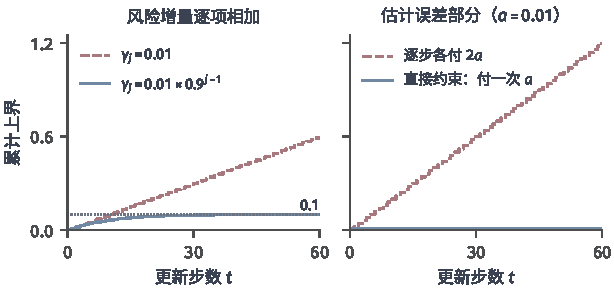
\includegraphics[width=104mm]{figures/06-foundations/02-learning-theory/matplotlib/lt9-forgetting-accumulation/figure.pdf}
 \caption{累计遗忘上界随更新步数的变化。左图：每步风险增量上界为常数0.01（虚线）时线性增长；按$0.9^{j-1}$递减（实线）时累计和小于0.1（点线）。右图：只看估计误差，取$a=0.01$，每步用经验增量控制都付$2a$时累计为$2at$（虚线），直接约束最终模型的历史经验风险只付一次$a$（实线）。数值为解析教学构造。}
 \label{fig:lt9-forgetting-accumulation}
\end{figure}
风险增量本身不可观察，要由历史经验比较与一致估计联系起来。假定第$i$阶段保留的信息给出估计$\widehat R_i$，并已证明对后续\emph{所有可能输出}的候选同时有$|R_i(h)-\widehat R_i(h)|\leq a_i$。对更新前后的两个模型分别使用偏差界，
\[
 R_i(h^{(j)})-R_i(h^{(j-1)})
 \leq\widehat R_i(h^{(j)})-\widehat R_i(h^{(j-1)})+2a_i .
\]
所以在经验上限制风险增量，还要支付历史估计的误差。若每次都用同一个$2a_i$累加，$t-i$步后估计误差部分为$2(t-i)a_i$，见图~\ref{fig:lt9-forgetting-accumulation}右图；它随步数增长，即使每步经验增量都为零。另一种做法是直接约束最终模型：若能让$h^{(t)}$的历史经验风险满足$\widehat R_i(h^{(t)})\leq\theta$，则$R_i(h^{(t)})\leq\theta+a_i$，只付一次$a_i$，不必把每次更新的$2a_i$加起来。第~\ref{sec:continual-fixed-candidates}节的两个构造正是这种直接控制。逐步累加与直接约束的差别说明，不能把每一步的保证机械地视为长期保证。

上面的转换必须覆盖反复选出的模型。只对一个预先固定模型成立的点态估计，不能直接用于之后根据同一批历史信息选出的许多模型；保留的回放样本若被用来反复挑选更新方向，偏差控制就要覆盖全部可能的输出。保留一个小回放集、限制参数变化或约束更新方向，都需要在相应的模型和抽样条件下进一步证明它们怎样控制历史总体风险；当前训练误差下降本身不提供这一结论。数据存在时间相关或模型反馈时，损失估计所需的独立性也要重新检查。参数化模型中任务顺序、参数规模和更新方向怎样影响遗忘，需要结合具体模型说明；已有过参数化线性模型的研究分析了任务相似性、顺序与遗忘及泛化的关系，其证明条件不能直接推广为任意神经网络的保证\scite{lin2023forgetting}。

\section{本章小结}
\label{sec:transfer-learning-summary}

本章开头的三个问题，分别对应同分布学习中断开的一条联系，也分别需要一种额外的信息联系。分布变化时，需要从源观测约束目标风险：协变量偏移下靠共享条件标签规律与覆盖，把目标风险改写为按输入加权的源期望；标签偏移下靠不变的类内分布与可识别的混合比例，改写为按类别加权的源期望；分歧散度路线则用源风险、可观察的输入差异和不可观察的共同错误$\lambda$给出上界。没有这样的联系时，相同的观测可以对应不兼容的目标决策（定理~\ref{thm:transfer-nonidentifiability}），或者目标输入根本不在源域出现（定理~\ref{thm:covariate-coverage-failure}），增加同类样本都无济于事。没有目标数据时，逐目标域保证依赖共同Bayes候选与统一覆盖，环境平均保证依赖独立环境的数量；两种承诺的量词不同，不能互推。任务变化时，需要旧知识保留目标决策所需的信息：硬类别丢失移动阈值所需的概率，固定表示可能留下不可消除的近似差$a_T(K)$，而保留概率可以不用目标标签就控制新代价下的超额风险。历史访问受限时，需要在存储限制下保留未来选择的依据：累计损失支持历史平均目标，前缀最大经验超额风险支持逐域目标，而保留任意独立标签串需要随阶段数线性增长的比特数。复杂度与稳定性工具控制这些路线中的统计代价，它们不能补造缺失的标签联系或历史信息。

综合来看，一个迁移或持续学习的结论要同时说明五件事：可识别性回答可见信息能否确定好决策，表达兼容回答是否存在满足全部要求的共同模型，样本误差回答有限数据能否估计所需风险，求解代价回答算法离经验最优还有多远，记忆预算回答状态能否保留后续选择所需的区别。本章的每个正面构造和下界都针对一个明确的协议：反馈有哪些、比较基准是什么、候选是否固定。协议改变以后，结论需要重新检查，例如允许目标标签、提供环境身份、改变历史权重或新增候选，都会改变哪些反例成立、哪些构造仍然够用。

\paragraph{扩展阅读}
Ben-David等人的领域自适应分析把源风险、输入分歧与共同错误联系起来；其不可学习性研究适合与本章反例对照，检查哪些可观察相似性仍不足以支持目标保证\scite{bendavid2010adaptation,bendavid2010impossibility}。标签偏移下比例的识别与估计，可参考利用黑盒分类器混淆矩阵反解比例的工作，注意其可逆性与类内分布不变的条件\scite{ket-lipton2018-labelshift}。

Tripuraneni、Jordan与Jin研究源任务的多样性如何支持共享表示及新任务的样本效率；Maurer、Pontil与Romera-Paredes从多任务表示学习分析共享结构的收益。阅读时应分别核对任务抽样、表示假设和新任务反馈，不能把这些结果理解为对任意任务变化的统一承诺\scite{tripuraneni2020diversity,maurer2016representation}。

Chen、Papadimitriou与Peng从PAC框架研究持续学习的记忆需求，以及多次访问任务带来的改变，可用于比较一次读取、重访与状态容量的关系。Lin等人在过参数化线性模型下分析遗忘与泛化，适合进一步理解任务联系、参数规模和顺序为何需要同时进入理论条件\scite{chen2022memory,lin2023forgetting}。
